% This is the Reed College LaTeX thesis template. Most of the work
% for the document class was done by Sam Noble (SN), as well as this
% template. Later comments etc. by Ben Salzberg (BTS). Additional
% restructuring and APA support by Jess Youngberg (JY).
% Your comments and suggestions are more than welcome; please email
% them to cus@reed.edu
%
% See http://web.reed.edu/cis/help/latex.html for help. There are a
% great bunch of help pages there, with notes on
% getting started, bibtex, etc. Go there and read it if you're not
% already familiar with LaTeX.
%
% Any line that starts with a percent symbol is a comment.
% They won't show up in the document, and are useful for notes
% to yourself and explaining commands.
% Commenting also removes a line from the document;
% very handy for troubleshooting problems. -BTS

% As far as I know, this follows the requirements laid out in
% the 2002-2003 Senior Handbook. Ask a librarian to check the
% document before binding. -SN

%%
%% Preamble
%%
% \documentclass{<something>} must begin each LaTeX document
\documentclass[12pt,twoside]{reedthesis}
% Packages are extensions to the basic LaTeX functions. Whatever you
% want to typeset, there is probably a package out there for it.
% Chemistry (chemtex), screenplays, you name it.
% Check out CTAN to see: http://www.ctan.org/
%%
\usepackage{graphicx,latexsym}
\usepackage{amsmath}
\usepackage{amssymb,amsthm}
\usepackage{longtable,booktabs,setspace}
\usepackage{chemarr} %% Useful for one reaction arrow, useless if you're not a chem major
\usepackage[hyphens]{url}
% Added by CII
\usepackage{hyperref}
\usepackage{lmodern}
\usepackage{float}
\floatplacement{figure}{H}
% End of CII addition
\usepackage{rotating}

% Next line commented out by CII
%%% \usepackage{natbib}
% Comment out the natbib line above and uncomment the following two lines to use the new
% biblatex-chicago style, for Chicago A. Also make some changes at the end where the
% bibliography is included.
%\usepackage{biblatex-chicago}
%\bibliography{thesis}


% Added by CII (Thanks, Hadley!)
% Use ref for internal links
\renewcommand{\hyperref}[2][???]{\autoref{#1}}
\def\chapterautorefname{Chapter}
\def\sectionautorefname{Section}
\def\subsectionautorefname{Subsection}
% End of CII addition

% Added by CII
\usepackage{caption}
\captionsetup{width=5in}
% End of CII addition

% \usepackage{times} % other fonts are available like times, bookman, charter, palatino

% Syntax highlighting #22
  \usepackage{color}
  \usepackage{fancyvrb}
  \newcommand{\VerbBar}{|}
  \newcommand{\VERB}{\Verb[commandchars=\\\{\}]}
  \DefineVerbatimEnvironment{Highlighting}{Verbatim}{commandchars=\\\{\}}
  % Add ',fontsize=\small' for more characters per line
  \usepackage{framed}
  \definecolor{shadecolor}{RGB}{248,248,248}
  \newenvironment{Shaded}{\begin{snugshade}}{\end{snugshade}}
  \newcommand{\KeywordTok}[1]{\textcolor[rgb]{0.13,0.29,0.53}{\textbf{#1}}}
  \newcommand{\DataTypeTok}[1]{\textcolor[rgb]{0.13,0.29,0.53}{#1}}
  \newcommand{\DecValTok}[1]{\textcolor[rgb]{0.00,0.00,0.81}{#1}}
  \newcommand{\BaseNTok}[1]{\textcolor[rgb]{0.00,0.00,0.81}{#1}}
  \newcommand{\FloatTok}[1]{\textcolor[rgb]{0.00,0.00,0.81}{#1}}
  \newcommand{\ConstantTok}[1]{\textcolor[rgb]{0.00,0.00,0.00}{#1}}
  \newcommand{\CharTok}[1]{\textcolor[rgb]{0.31,0.60,0.02}{#1}}
  \newcommand{\SpecialCharTok}[1]{\textcolor[rgb]{0.00,0.00,0.00}{#1}}
  \newcommand{\StringTok}[1]{\textcolor[rgb]{0.31,0.60,0.02}{#1}}
  \newcommand{\VerbatimStringTok}[1]{\textcolor[rgb]{0.31,0.60,0.02}{#1}}
  \newcommand{\SpecialStringTok}[1]{\textcolor[rgb]{0.31,0.60,0.02}{#1}}
  \newcommand{\ImportTok}[1]{#1}
  \newcommand{\CommentTok}[1]{\textcolor[rgb]{0.56,0.35,0.01}{\textit{#1}}}
  \newcommand{\DocumentationTok}[1]{\textcolor[rgb]{0.56,0.35,0.01}{\textbf{\textit{#1}}}}
  \newcommand{\AnnotationTok}[1]{\textcolor[rgb]{0.56,0.35,0.01}{\textbf{\textit{#1}}}}
  \newcommand{\CommentVarTok}[1]{\textcolor[rgb]{0.56,0.35,0.01}{\textbf{\textit{#1}}}}
  \newcommand{\OtherTok}[1]{\textcolor[rgb]{0.56,0.35,0.01}{#1}}
  \newcommand{\FunctionTok}[1]{\textcolor[rgb]{0.00,0.00,0.00}{#1}}
  \newcommand{\VariableTok}[1]{\textcolor[rgb]{0.00,0.00,0.00}{#1}}
  \newcommand{\ControlFlowTok}[1]{\textcolor[rgb]{0.13,0.29,0.53}{\textbf{#1}}}
  \newcommand{\OperatorTok}[1]{\textcolor[rgb]{0.81,0.36,0.00}{\textbf{#1}}}
  \newcommand{\BuiltInTok}[1]{#1}
  \newcommand{\ExtensionTok}[1]{#1}
  \newcommand{\PreprocessorTok}[1]{\textcolor[rgb]{0.56,0.35,0.01}{\textit{#1}}}
  \newcommand{\AttributeTok}[1]{\textcolor[rgb]{0.77,0.63,0.00}{#1}}
  \newcommand{\RegionMarkerTok}[1]{#1}
  \newcommand{\InformationTok}[1]{\textcolor[rgb]{0.56,0.35,0.01}{\textbf{\textit{#1}}}}
  \newcommand{\WarningTok}[1]{\textcolor[rgb]{0.56,0.35,0.01}{\textbf{\textit{#1}}}}
  \newcommand{\AlertTok}[1]{\textcolor[rgb]{0.94,0.16,0.16}{#1}}
  \newcommand{\ErrorTok}[1]{\textcolor[rgb]{0.64,0.00,0.00}{\textbf{#1}}}
  \newcommand{\NormalTok}[1]{#1}

% To pass between YAML and LaTeX the dollar signs are added by CII
\title{Developing A Tool to Uncover The Mysterious New York City Through Taxi
Trip Records}
\author{Wencong (Priscilla) Li}
% The month and year that you submit your FINAL draft TO THE LIBRARY (May or December)
\date{May 2018}
\division{}
\advisor{Benjamin Baumer}
\institution{Smith College}
\degree{Bachelor of Arts}
%If you have two advisors for some reason, you can use the following
% Uncommented out by CII
\altadvisor{Jordan Crouser}
% End of CII addition

%%% Remember to use the correct department!
\department{Statistical and Data Sciences}
% if you're writing a thesis in an interdisciplinary major,
% uncomment the line below and change the text as appropriate.
% check the Senior Handbook if unsure.
%\thedivisionof{The Established Interdisciplinary Committee for}
% if you want the approval page to say "Approved for the Committee",
% uncomment the next line
%\approvedforthe{Committee}

% Added by CII
%%% Copied from knitr
%% maxwidth is the original width if it's less than linewidth
%% otherwise use linewidth (to make sure the graphics do not exceed the margin)
\makeatletter
\def\maxwidth{ %
  \ifdim\Gin@nat@width>\linewidth
    \linewidth
  \else
    \Gin@nat@width
  \fi
}
\makeatother

\renewcommand{\contentsname}{Table of Contents}
% End of CII addition

\setlength{\parskip}{0pt}

% Added by CII
  %\setlength{\parskip}{\baselineskip}
  \usepackage[parfill]{parskip}

\providecommand{\tightlist}{%
  \setlength{\itemsep}{0pt}\setlength{\parskip}{0pt}}

\Acknowledgements{
\chapter*{Acknowledgements}\label{acknowledgements}
\addcontentsline{toc}{chapter}{Acknowledgements}

I would love to thank my thesis advisor Benjamin Baumer, Assistant
Professor of Statistical and Data Sciences at Smith College, for
encouraging me to chanllenge myself and and guiding me through this
project. I also want to thank all my friedns and my roommates for their
love and support.
}

\Dedication{

}

\Preface{

}

\Abstract{
\chapter*{Abstract}\label{abstract}
\addcontentsline{toc}{chapter}{Abstract}

The New York City Taxi Cabs are widely recognized as the icons of New
York City. The New York City Taxi \& Limousine Commission provide
publicly accessible yellow and green taxi trip records for people to do
research with. Each taxi trip record is like a little piece of a
gigantic puzzle, and all together they draw a picture of what is
happening in New York City every day. This thesis presents a more
efficient and easy-to-use way for users to retrieve information of both
New York City taxi trip record and trip records of other ridesharing
services in New York City, such as Uber and Lyft. By focusing on New
York City's iconic yellow taxi's trip records, we investigate social and
taxi pricing questions. Additionally, this thesis illustrates a way for
taxi drivers to better understand where the customers are and where the
customers try to go.
}

% End of CII addition
%%
%% End Preamble
%%
%

\usepackage{amsthm}
\newtheorem{theorem}{Theorem}[chapter]
\newtheorem{lemma}{Lemma}[chapter]
\theoremstyle{definition}
\newtheorem{definition}{Definition}[chapter]
\newtheorem{corollary}{Corollary}[chapter]
\newtheorem{proposition}{Proposition}[chapter]
\theoremstyle{definition}
\newtheorem{example}{Example}[chapter]
\theoremstyle{definition}
\newtheorem{exercise}{Exercise}[chapter]
\theoremstyle{remark}
\newtheorem*{remark}{Remark}
\newtheorem*{solution}{Solution}
\begin{document}

% Everything below added by CII
  \maketitle

\frontmatter % this stuff will be roman-numbered
\pagestyle{empty} % this removes page numbers from the frontmatter
  \begin{acknowledgements}
    \chapter*{Acknowledgements}\label{acknowledgements}
    \addcontentsline{toc}{chapter}{Acknowledgements}
    
    I would love to thank my thesis advisor Benjamin Baumer, Assistant
    Professor of Statistical and Data Sciences at Smith College, for
    encouraging me to chanllenge myself and and guiding me through this
    project. I also want to thank all my friedns and my roommates for their
    love and support.
  \end{acknowledgements}

  \hypersetup{linkcolor=black}
  \setcounter{tocdepth}{2}
  \tableofcontents

  \listoftables

  \listoffigures
  \begin{abstract}
    \chapter*{Abstract}\label{abstract}
    \addcontentsline{toc}{chapter}{Abstract}
    
    The New York City Taxi Cabs are widely recognized as the icons of New
    York City. The New York City Taxi \& Limousine Commission provide
    publicly accessible yellow and green taxi trip records for people to do
    research with. Each taxi trip record is like a little piece of a
    gigantic puzzle, and all together they draw a picture of what is
    happening in New York City every day. This thesis presents a more
    efficient and easy-to-use way for users to retrieve information of both
    New York City taxi trip record and trip records of other ridesharing
    services in New York City, such as Uber and Lyft. By focusing on New
    York City's iconic yellow taxi's trip records, we investigate social and
    taxi pricing questions. Additionally, this thesis illustrates a way for
    taxi drivers to better understand where the customers are and where the
    customers try to go.
  \end{abstract}

\mainmatter % here the regular arabic numbering starts
\pagestyle{fancyplain} % turns page numbering back on

\chapter{Introduction}\label{introduction}

\section{Motivation}\label{motivation}

Working with medium data in R is not an easy task. Loading medium-sized
data into R environment takes a long time and might crush an R session.
Creating a user-friendly platform that allows R users to easily work
with medium data is my motivation. There are a lot of interesting data
that are needed to be explored. In my study, I focus on New York City
taxicab data, because there is so much that could be learned from
taxicab trip records.

New York City taxi drivers, passengers, and NYC Taxi \& Limousine
Commission are the three parties who are closely involved in the NYC
taxi industry. Each party has its own needs. Better understanding the
needs of the three parties and provide solutions to better satisfy their
needs are what I am hooping to be the result of this thiesis.
\begin{center}\rule{0.5\linewidth}{\linethickness}\end{center}

\section{Background}\label{background}

\subsection{Yellow Taxi}\label{yellow-taxi}

The Yellow Cabs are widely recognized as the icons of New York City. NYC
Taxicabs are operated by private firms and licensed by the New York City
Taxi and Limousine Commission (TLC). TLC issues medallions to taxicabs,
and every taxicab must have a medallion to operate. There were 13,437
yellow medallion taxicabs licenses in 2014, and taxi patronage has
declined since 2011 because of the competition caused by rideshare
services.

\subsection{Green Taxi}\label{green-taxi}

The apple green taxicabs in New York City are called Boro taxis and they
are allowed to only pick up passengers in outer boroughs and in
Manhattan above East 96th and West 110th Streets. Historically, only the
yellow medallion taxicabs were allowed to pick up passengers on the
street. However, since 95\% of yellow taxi pick-ups occurred in
Manhattan to the South of 96th Street and at the two airports, Five
Borough Taxi Plan was started to allow green taxis to fill in the gap in
outer boroughs.

\subsection{Uber}\label{uber}

Uber Technologies Inc., famously known as Uber, is an American
technology company that operates private cars worldwide. Uber drivers
use their own cars, instead of corporate-owned vehicles, to drive with
Uber. In NYC, Uber uses `upfront pricing'', meaning that riders are
informed about the fares that they will pay before requesting a ride,
and gratuity is not required. Riders are given the opportunity to
compare different transportation fares before making their decisions on
which one to choose. Uber NYC was launched in May 2011, and it only took
5 years to have its growth to plateau.

\subsection{Lyft}\label{lyft}

Similar to Uber, Lyft is also an on-demand transportation company, and
it operates the Lyft car transportation mobile app. Lyft is the main
competitor of Uber, and it came into market in July 2014 in New York
City.
\begin{center}\rule{0.5\linewidth}{\linethickness}\end{center}

\section{Literature Review}\label{literature-review}
\begin{center}\rule{0.5\linewidth}{\linethickness}\end{center}

\section{Contribution}\label{contribution}

\subsection{nyctaxi Package}\label{nyctaxi-package}

nyctaxi is an etl-dependent R package that help users to easily get
access to New York City Taxi, Uber and Lyft trip data through Extract,
Transform, and Load functions (ETL). This package facilitates ETL to
deal with medium data that are too big to store on a laptop. Users are
given the option to choose specific years and months as the input
parameters of the three ETL functions, and a populated SQL database will
be returned as the output. Users do not need to learn SQL queries, since
all user interaction is in R.

\subsection{Social Impact of NYC Taxi}\label{social-impact-of-nyc-taxi}

New York City taxi drivers, passengers, and NYC Taxi \& Limousine
Commission are the three parties who are closely involved in the NYC
taxi industry. Each party has its own needs: taxi drivers want to
maxmize their profit, and in order to do that, they need to maximize the
revenue while minimizing the cost. Taxi passengers want the cheapest and
most convenient way of transportantion. Since Uber and Lyft launched
their services in New York City, many consumers started to demand the
cheaper e-hail services. TLC wants to protect both taxi drivers and
passengers, and it creates policies to make NYC taxi more accessible to
consumers who really need this service. In this section, I think about
what each party wants and try to find a way for them to be better-off.

\subsection{Reproducible Research}\label{reproducible-research}

Reproducible research and open sources are the very first things that
Ben mentioned to me in the beginning of my honors project. As scholars
place more emphasis on the reproducibility of research studies, it is
essential for me to make my dat and code openly available for people to
eith redo my analysis or test my result.

\texttt{Knitr} and Github are used in my project to make my study
reproducible, ranging from the initial source to raw data to the package
I wrote to utlize the raw data to the statistical data analysis. I used
an Github Ripository called \texttt{thesisdown} to layout the basic
structure of my paper, this tool allows students to create reproducible
and dynamic techinical report in R Markdown. It also allows users to
embed R code and interactive applicationis, and output into PDF, Word,
ePub, or gitbook doocuments. \texttt{thesisdown} helps users to
efficiently put together any paper with similar format.

Github is used to store the scripts for \texttt{nyctaxi} and this
thesis. \texttt{nyctaxi} is available on CRAN for people to download and
install, and the source code for data analysis in this thesis is
available under the Github account of the author so that scholars can
easyil access the information that thery are interested in. In terms of
tables, figures, and anything included in the Appendix attached to this
thesis, scripts that are used to generate them are included in the
Github repository.

\chapter{Data and nyctaxi Package}\label{chapter1}

\section{Data and Storage}\label{data-and-storage}

The \texttt{nyctaxi} R package allows users to download, clean, and load
data into SQL databasses. There are four types of data that are
available for users to get access to, and they are New York City yellow
taxi trip data, NYC green taxi data, NYC uber trip data, and NYC lyft
data. Here is a summary of data that are available to users from 2014 to
2016.
\begin{figure}
\centering
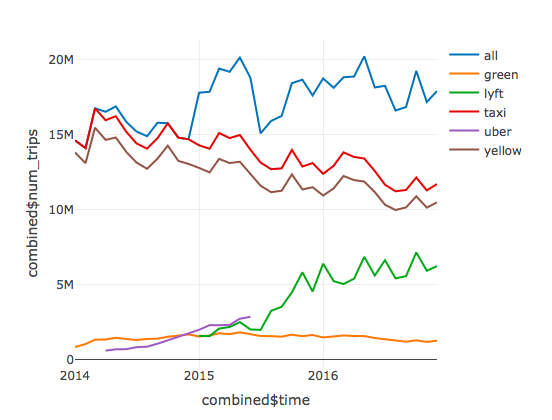
\includegraphics{figure/Num_trips_summary.png}
\caption{}
\end{figure}
\subsection{Yellow Taxi}\label{yellow-taxi-1}

The total size of all yellow taxi trip data \texttt{csv} files (from Jan
2010 to Dec 2016) is 191.38 GB, and NYC yellow taxi trip data from Jan
2009 to the most recent month can be found on NYC Taxi \& Limousine
Commission (TLC). The data were collected and provided to the NYC TLC by
technology providers authorized under the Taxicab \& Livery Passenger
Enhancement Programs (TPEP/LPEP).

The yellow taxi trip records include the following fields: pick-up and
drop-off dates/times, pick-up and drop-off locations, trip distances,
itemized fares, rate types, payment types, and driver-reported passenger
counts.

\subsection{Green Taxi}\label{green-taxi-1}

The total size of green taxi trip data \texttt{csv} files (from Aug 2013
to Dec 2016) is 7.8 GB, and green taxi trip data from Aug 2013 to the
most recent month can be downloaded from NYC Taxi \& Limousine
Commission (TLC). The data were collected and provided to the NYC TLC by
technology providers authorized under the Taxicab \& Livery Passenger
Enhancement Programs (TPEP/LPEP).

The green taxi trip records include the following fields: pick-up and
drop-off dates/times, pick-up and drop-off locations, trip distances,
itemized fares, rate types, payment types, and driver-reported passenger
counts.

\subsection{Uber}\label{uber-1}

The total size of Uber pick-up data (over 4.5 million from Apr to Sep
2014 and 14.3 million from Jan to June 2015) is 4.3 MB, and thanks to
FiveThirtyEight who obtained the data from NYC TLC by submitting a
Freedom of Information Law request on July 20, 2015, these data are now
open to public.

The 2014 Uber data contains four variables: Data/Time (the date and time
of the Uber pick-up), Lat (the latitude of the Uber pick-up), Lon (the
longitude of the Uber pick-up), and Base (the TLC base company code
affiliated with the Uber pickup).

The 2015 Uber data contains four variables: Dispatching\_base\_num (the
TLC base company code of the base that dispatched the Uber),
Pickup\_date (the date of the Uber pick-up), Affiliated\_base\_num (the
TLC base company code affiliated with the Uber pickup), and locationID
(the pick-up location ID affiliated with the Uber pickup).

\subsection{Lyft}\label{lyft-1}

The total size of weely-aggregated Lyft trip data (from Jan 2015 to Dec
2016) is 914.9 MB, and these data are open to public and
weekly-aggregated Lyft data from 2015 to the most recent week can be
found on NYC OpenData website.

\subsection{Storage}\label{storage}

The total size of all \texttt{csv} files of the four services is about
200 GB, and a laptop usually has memory less than or equal to 8GB.
Limited memory constrains the amount of data that can be loaded by a
personal computer. When users load data into R environment, R keeps them
in memory; when the amount of data loaded into R environment gets close
to the limit of a computer's memory, R becomes unresponsive or force
quit the current session. Therefore, better ways to work with data that
takes more space than 8 GB is needed. According to Weijia Zhang (2016),
comparing to RAM, hard disk is often used to store medium-sized data,
because it is affordable and are designed for storing large items
permanently. However, retrieving data from hard drives usually takes
about 1,000,000 times more time.

\section{ETL nyctaxi Package}\label{etl-nyctaxi-package}

etl is the parent package of nyctaxi. etl package provides a
CRAN-friendly framework that allows R users to work with medium data
without any knowledge in SQL database. The end result is a populated SQL
database, but the user interaction takes place solely within R. It has
three operations -extract, transfer, and load- which bring real-time
data into local or remote databases. etl-dependent packages make medium
data - too big to store in memory on a laptop- more accessible to a
wider audience. Additionally, etl-dependent packages use SQL translation
supported by dyplr.

nyctaxi was initially designed to work with New York City taxi data, but
later on Uber and Lyft data were added and the ETL functions are
modified to be specialized in working with these data. This package
compiled three major sources of hail service in New York City so that it
is convenient for users to compare and contrast the performance of these
three services.

This package inherits functions from many packages: etl, dplyr, DBI,
rlang, and stringr. Since SQL databases are good tools for medium data
analysis, ETL functions build connection to a SQL database at the back
end and convert R code automatically into SQL queries and send them to
the SQL database to get data tables containing data of each hail
service. Thus, users do not need to have any knowledge of SQL queries
and they can draw in any subsets of the data from the SQL database in R.

In general, extract.nyctaxi function download data of the four types of
hail service data (yellow taxi, green taxi, uber, and lyft) from the
corresponding sources. transform.nyctaxi uses different techniques to
clean all four types of data to get then ready for the next step.
extract.load loads the data user selected to a SQL database.

nyctaxi lives on the Comprehensive R Archive Network (CRAN), and
Packages can be installed with the install.packages() function in R.
\begin{Shaded}
\begin{Highlighting}[]
\CommentTok{# install the package}
\KeywordTok{install.packages}\NormalTok{(}\StringTok{"nyctaxi"}\NormalTok{)}

\CommentTok{# load the package}
\KeywordTok{library}\NormalTok{(nyctaxi)}
\end{Highlighting}
\end{Shaded}
Users need to create an etl object in order to apply the etl operations
to it, and only the name of the SQL database, working directory, and
type of SQL database need to be specified during initialization. If the
type of SQL database is not specified, a local RSQLite database will be
generated as default.
\begin{Shaded}
\begin{Highlighting}[]
\CommentTok{# initializing an etl object}
\NormalTok{db <-}\StringTok{ }\KeywordTok{src_mysql}\NormalTok{(}\StringTok{"nyctaxi"}\NormalTok{, }\DataTypeTok{user =} \StringTok{"urname"}\NormalTok{, }\DataTypeTok{host =} \StringTok{"host"}\NormalTok{, }
    \DataTypeTok{password =} \StringTok{"pw"}\NormalTok{)}
\NormalTok{taxi <-}\StringTok{ }\KeywordTok{etl}\NormalTok{(}\StringTok{"nyctaxi"}\NormalTok{, }\DataTypeTok{dir =} \StringTok{"~/Desktop/nyctaxi"}\NormalTok{, db)}
\end{Highlighting}
\end{Shaded}
In the example above, a folder called nyctaxi is created on the desktop
and a connection to a MySQL database is generated. In the procession of
initialization, a local folder contains two subfolders, \texttt{raw} and
\texttt{load}, are also created under the directory the user specifies.
\texttt{raw} folder stores data downloaded from online open sources, and
\texttt{load} folder stores cleaned CSV data files that are ready to be
loaded into SQL database. The ETL framework keeps data directly scraped
from online data sources in their original forms. In this way, the
original data is always available to users in case data corruption
happens in later stages.

After an etl object is created (nyctaxi is the etl object in this case),
four parameters are needed to specify the data that users want: (1) obj:
an etl object (2) years: a numeric vector giving the years. The default
is the most recent year. (3) months: a numeric vector giving the months.
The default is January to December. (4) type: a character variable
giving the type of data the user wants to download. There are four
types: yellow, green, uber, and lyft. The default is yellow.

\subsection{Taxi zone shapefile attached to nyctaxi R
package}\label{taxi-zone-shapefile-attached-to-nyctaxi-r-package}

\section{Extract}\label{extract}

etl\_extract.nyctaxi allows users to download New York City yellow taxi,
green taxi, Uber, and Lyft data that are specific to their month of
interest.

\subsection{Yellow Taxi}\label{yellow-taxi-2}

\subsection{Green Taxi}\label{green-taxi-2}

\subsection{Uber}\label{uber-2}

\subsection{Lyft}\label{lyft-2}

\section{Transform}\label{transform}

etl\_extract.nyctaxi allows users to transform New York City yellow
taxi, green taxi, Uber, and Lyft data into forms that are meaningful to
users.

\subsection{Yellow Taxi}\label{yellow-taxi-3}

\subsection{Green Taxi}\label{green-taxi-3}

\subsection{Uber}\label{uber-3}

\subsection{Lyft}\label{lyft-3}

\section{Load}\label{load}

etl\_extract.nyctaxi allows users to load New York City yellow taxi,
green taxi, Uber, and Lyft data into different data tables in a SQL
database.

\subsection{Yellow Taxi}\label{yellow-taxi-4}

\subsection{Green Taxi}\label{green-taxi-4}

\subsection{Uber}\label{uber-4}

\subsection{Lyft}\label{lyft-4}

\section{SQL Database Initialization}\label{sql-database-initialization}

\subsection{Yellow Taxi}\label{yellow-taxi-5}

\subsection{Green Taxi}\label{green-taxi-5}

\subsection{Uber}\label{uber-5}

\subsection{Lyft}\label{lyft-5}

\section{New Yoek City Hail Service
Summary}\label{new-yoek-city-hail-service-summary}

\section{Source Code}\label{source-code}

\subsection{ETL Extract}\label{etl-extract}
\begin{verbatim}
opts_chunk$set(tidy.opts=list(width.cutoff=60))

etl_extract.etl_nyctaxi <- 
  function(obj, 
years = as.numeric(format(Sys.Date(),'%Y')), 
                                    months = 1:12, 
                                    type  = "yellow",...) {
  #TAXI YELLOW-------------------------
  taxi_yellow <- function(obj, years, months,...) {
    message("Extracting raw yellow taxi data...")
    remote <- etl::valid_year_month(years, months, 
    begin = "2009-01-01") %>%
      mutate_(src = 
  ~file.path("https://s3.amazonaws.com/nyc-tlc/trip+data", 
                               paste0("yellow", "_tripdata_", year, "-",
                      stringr::str_pad(month, 2, "left", "0"), ".csv"))) 
    tryCatch(expr = etl::smart_download(obj, remote$src, ...),
             error = function(e){warning(e)}, 
             finally = warning("Only the following data are availabel on
                                TLC: Yellow taxi data: 2009 Jan - 
                               last month"))} 
  #TAXI GREEN----------------------
  taxi_green <- function(obj, years, months,...) {
    message("Extracting raw green taxi data...")
    remote <- etl::valid_year_month(years, months, begin = "2013-08-01") %>%
      mutate_(src = 
                ~file.path("https://s3.amazonaws.com/nyc-tlc/trip+data", 
                               paste0("green", "_tripdata_", year, "-",
                          stringr::str_pad(month, 2, "left", "0"), ".csv")))
    tryCatch(expr = etl::smart_download(obj, remote$src, ...),
             error = function(e){warning(e)}, 
             finally = warning("Only the following data are availabel on TLC:
                               Green taxi data: 2013 Aug - last month"))} 
  #UBER--------------------------------
  uber <- function(obj, years, months,...) {
    message("Extracting raw uber data...")
    raw_month_2014 <- etl::valid_year_month(years = 2014, months = 4:9)
    raw_month_2015 <- etl::valid_year_month(years = 2015, months = 1:6)
    raw_month <- bind_rows(raw_month_2014, raw_month_2015)
    path = "https://raw.githubusercontent.com/
    fivethirtyeight/uber-tlc-foil-response/master/uber-trip-data"
    remote <- etl::valid_year_month(years, months)
    remote_small <- intersect(raw_month, remote)
    if (2015 %in% remote_small$year && !(2014 %in% remote_small$year)){
      #download 2015 data
      message("Downloading Uber 2015 data...")
      etl::smart_download(obj, "https://github.com/fivethirtyeight/
                          uber-tlc-foil-response/raw/master/
                    uber-trip-data/uber-raw-data-janjune-15.csv.zip",...)}
    else if (2015 %in% remote_small$year && 2014 %in% remote_small$year) {
      #download 2015 data
      message("Downloading Uber 2015 data...")
      etl::smart_download(obj, "https://github.com/fivethirtyeight/
                        uber-tlc-foil-response/raw/master/uber-trip-data
                          /uber-raw-data-janjune-15.csv.zip",...)
      #download 2014 data
      small <- remote_small %>%
        filter_(~year == 2014) %>%
        mutate_(month_abb = ~tolower(month.abb[month]),
                src = ~file.path(path,
                paste0("uber-raw-data-",month_abb,
                substr(year,3,4),".csv")))
      message("Downloading Uber 2014 data...")
      etl::smart_download(obj, small$src,...) 
    } else if (2014 %in% remote_small$year && 
    !(2015 %in% remote_small$year)) {
      message("Downloading Uber 2014 data...")
      #file paths
      small <- remote_small %>%
        mutate_(month_abb = 
                  ~tolower(month.abb[month]),
                src = ~file.path(path,
                paste0("uber-raw-data-",month_abb,
                substr(year,3,4),".csv")))
      etl::smart_download(obj, small$src,...)}
    else {warning("The Uber data you requested are 
                  not currently available. Only data
                  from 2014/04-2014/09 and 2015/01-
                  2015/06 are available...")}
    } 
  #LYFT----------------------------------
  lyft <- function(obj, years, months,...){
    message("Extracting raw lyft data...")
    #check if the week is valid
    valid_months <- etl::valid_year_month(years, months,
    begin = "2015-01-01")
    base_url = "https://data.cityofnewyork.us/
    resource/edp9-qgv4.csv"
    valid_months <- valid_months %>%
      mutate_(new_filenames = 
                ~paste0("lyft-", year, ".csv")) %>%
      mutate_(drop = TRUE)
    #only keep one data set per year
    year <- valid_months[1,1]
    n <- nrow(valid_months)
    for (i in 2:n) {
      if(year == valid_months[i-1,1]) {
        valid_months[i,6] <- FALSE
        year <- valid_months[i+1,1]
      } else {
        valid_months[i,6] <- TRUE
        year <- valid_months[i+1,1]}
      }
    row_to_keep = valid_months$drop
    valid_months <- valid_months[row_to_keep,]
    
    #download lyft files, try two different methods
    first_try<-tryCatch(
      download_nyc_data(obj, base_url, valid_months$year, 
      n = 50000, names = valid_months$new_filenames),
      error = function(e){warning(e)},
      finally = 'method = "libcurl" fails')
  }
  
  if (type == "yellow"){taxi_yellow(obj, years, months,...)} 
  else if (type == "green"){taxi_green(obj, years, months,...)}
  else if (type == "uber"){uber(obj, years, months,...)}
  else if (type == "lyft"){lyft(obj, years, months,...)}
  else {message("The type you chose does not exit...")}
  
  invisible(obj)
}
\end{verbatim}
\subsection{ETL Transform}\label{etl-transform}
\begin{verbatim}
opts_chunk$set(tidy.opts=list(width.cutoff=60))
etl_transform.etl_nyctaxi <- function(obj, 
                          years = as.numeric(format(Sys.Date(),'%Y')), 
                          months = 1:12, 
                          type  = "yellow",...) {
  #TAXI YELLOW-----------------------------
  taxi_yellow <- function(obj, years, months) {
    message("Transforming yellow taxi data from raw to 
            load directory...")
    #create a df of file path of the files that the user wants to transform
    remote <- etl::valid_year_month(years, months, 
    begin = "2009-01-01") %>%
      mutate_(src = ~file.path(attr(obj, "raw_dir"), 
      paste0("yellow", "_tripdata_", year, "-",
      stringr::str_pad(month, 2, "left", "0"), ".csv"))) 
    #create a df of file path of the files that are in the raw directory
    src <- list.files(attr(obj, "raw_dir"), "yellow", full.names = TRUE)
    src_small <- intersect(src, remote$src)
    #Move the files
    in_raw <- basename(src_small)
    in_load <- basename(list.files(attr(obj, "load_dir"), "yellow", 
    full.names = TRUE))
    file_remian <- setdiff(in_raw,in_load)
    file.copy(file.path(attr(obj, "raw_dir"),file_remian),
              file.path(attr(obj, "load_dir"),file_remian) )}
  #TAXI GREEN-----------------------------
  taxi_green <- function(obj, years, months) {
    message("Transforming green taxi data from raw 
            to load directory...")
    #create a df of file path of the files that the user wants to transform
    remote <- etl::valid_year_month(years, months, 
    begin = "2013-08-01") %>%
      mutate_(src = ~file.path(attr(obj, "raw_dir"), 
      paste0("green", "_tripdata_", year, "-",
      stringr::str_pad(month, 2, "left", "0"), ".csv"))) 
    #create a df of file path of the files that are in the raw directory
    src <- list.files(attr(obj, "raw_dir"), "green", full.names = TRUE)
    src_small <- intersect(src, remote$src)
    #Clean the green taxi data files
    #get rid of 2nd blank row
    if (length(src_small) == 0){
      message("The files you requested are not available 
              in the raw directory.")
    } else{
      #a list of the ones that have a 2nd blank row
      remote_green_1 <- remote %>% filter_(~year != 2015)
      src_small_green_1 <- intersect(src, remote_green_1$src)
      # check that the sys support command line, 
      #and then remove the blank 2nd row
      if(length(src_small_green_1) != 0) {
        if (.Platform$OS.type == "unix"){
          cmds_1 <- paste("sed -i -e '2d'", src_small_green_1)
          lapply(cmds_1, system)
        } else {
          message("Windows system does not 
          currently support removing the 2nd blank row
          in the green taxi datasets. This might affect 
          loading data into SQL...")}
        }else {
          "You did not request for any 
          green taxi data, or all the green
          taxi data you requested are cleaned."}
      #fix column number
      remote_green_2 <- remote %>%
        filter_(~year %in% c(2013, 2014, 2015)) %>%
        mutate_(keep = 
                  ~ifelse(year %in% c(2013,2014), 20,21),
                new_file = 
                  ~paste0("green_tripdata_", year, "_", 
                      stringr::str_pad(month, 2, "left", "0"),
                                   ".csv"))
      src_small_green_2 <- intersect(src, remote_green_2$src)
      src_small_green_2_df <- data.frame(src_small_green_2) 
      names(src_small_green_2_df) <- "src"
      src_small_green_2_df <- inner_join(src_small_green_2_df, 
      remote_green_2, by = "src")
      src_small_green_2_df <- src_small_green_2_df %>%
        mutate(cmds_2 = paste("cut -d, -f1-", keep," ",src, " > ",
        attr(obj, "raw_dir"),"/green_tripdata_", 
        year, "_", stringr::str_pad(month, 2, "left", "0"),".csv", 
        sep = ""))
      #remove the extra column
      if(length(src_small_green_2) != 0) {
        if (.Platform$OS.type == "unix"){
          lapply(src_small_green_2_df$cmds_2, system)} 
        else {
          message("Windows system does not currently 
          support removing the 2nd blank row 
          in the green taxi datasets. This might 
          affect loading data into SQL...")}
        }else {
          "All the green taxi data you
          requested are in cleaned formats."}
      #Find the files paths of the files that need to be transformed
      file.rename(file.path(dirname(src_small_green_2_df$src),
                            src_small_green_2_df$new_file), 
                  file.path(attr(obj, "load_dir"),
                  basename(src_small_green_2_df$src)))
      #Move the files
      in_raw <- basename(src_small)
      in_load <- basename(list.files(attr(obj, "load_dir"), 
      "green", full.names = TRUE))
      file_remian <- setdiff(in_raw,in_load)
      file.copy(file.path(attr(obj, "raw_dir"),file_remian), 
      file.path(attr(obj, "load_dir"),file_remian) )}}
  #UBER--------------------------------
  uber <- function(obj) {
    message("Transforming uber data from raw to load directory...")
    #creat a list of 2014 uber data file directory
    uber14_list <- list.files(path = attr(obj, "raw_dir"), 
    pattern = "14.csv")
    uber14_list <- data.frame(uber14_list)
    uber14_list <- uber14_list %>% mutate_(file_path = 
    ~file.path(attr(obj, "raw_dir"), uber14_list))
    uber14file <- lapply(uber14_list$file_path, readr::read_csv)
    n <- length(uber14file)
    if (n == 1) {
      uber14 <- data.frame(uber14file[1])
    } else if (n == 2) {
      uber14 <- bind_rows(uber14file[1], uber14file[2])
    } else if (n > 2) {
      uber14 <- bind_rows(uber14file[1], uber14file[2])
      for (i in 3:n){uber14 <- bind_rows(uber14, uber14file[i])}
    }
    substrRight <- function(x, n){substr(x, nchar(x)-n+1, nchar(x))}
    uber14_datetime <- uber14 %>%
      mutate(date = gsub( " .*$", "", `Date/Time`), 
      len_date = nchar(date), 
             time = sub('.*\\ ', '', `Date/Time`))
    uber14_datetime <- uber14_datetime %>%
      mutate(month = 
               substr(`Date/Time`, 1, 1),
             day = ifelse(len_date == 8, 
             substr(`Date/Time`, 3,3),substr(`Date/Time`, 3,4)),
             pickup_date = 
               lubridate::ymd_hms(paste0("2014-", month, "-", 
                                         day, " ", time)))
    uber14_df <- uber14_datetime[-c(1,5:9)]
    
    #2015
    zipped_uberfileURL <- file.path(attr(obj, "raw_dir"),
    "uber-raw-data-janjune-15.csv.zip")
    raw_month_2015 <- etl::valid_year_month(years = 2015, months = 1:6)
    remote_2015 <- etl::valid_year_month(years, months)
    remote_small_2015 <- inner_join(raw_month_2015, remote_2015)
    if(file.exists(zipped_uberfileURL) && 
       nrow(remote_small_2015) != 0){
      utils::unzip(zipfile = zipped_uberfileURL,unzip = "internal",
      exdir = file.path(tempdir(), "uber-raw-data-janjune-15.csv.zip"))
      uber15 <- readr::read_csv(file.path(tempdir(),
      "uber-raw-data-janjune-15.csv.zip",
      "uber-raw-data-janjune-15.csv"))}
    
    names(uber14_df) <- c("lat", "lon", "affiliated_base_num", 
    "pickup_date")
    names(uber15) <- tolower(names(uber15))
    uber <- bind_rows(uber14_df, uber15)
    utils::write.csv(uber, file.path(tempdir() ,"uber.csv"))
    if(nrow(uber) != 0) {
      if (.Platform$OS.type == "unix"){cmds_3 <- 
      paste("cut -d, -f2-7",file.path(tempdir(),"uber.csv"), " > ", 
      file.path(attr(obj, "load_dir"),"uber.csv"))
        lapply(cmds_3, system)
      } else {
        message("Windows system does not currently 
        support removing the 2nd blank row 
        in the green taxi datasets. This might
        affect loading data into SQL...")}
      }else {
        "You did not request for any 
        green taxi data, or all the green 
        taxi data you requested are cleaned."}
    }
  #LYFT--------------------------------
  lyft <- function(obj, years, months){
    valid_months <- etl::valid_year_month(years, months = 1, 
    begin = "2015-01-01")
    message("Transforming lyft data from raw to load directory...")
    src <- list.files(attr(obj, "raw_dir"), "lyft", full.names = TRUE)
    src_year <- valid_months %>% distinct_(~year)
    remote <- data_frame(src)
    remote <- remote %>%
      mutate_(lcl = ~file.path(attr(obj, "load_dir"),basename(src)),
              basename = ~basename(src), year = ~substr(basename,6,9))
    class(remote$year) <- "numeric"
    remote <- inner_join(remote,src_year, by = "year" )
    for(i in 1:nrow(remote)) {
        datafile <- readr::read_csv(remote$src[i])
        readr::write_delim(datafile, path = remote$lcl[i], 
        delim = "|", na = "")}}
  
  #transform the data from raw to load
  if (type == "yellow"){taxi_yellow(obj, years, months)} 
  else if (type == "green"){taxi_green(obj, years, months)}
  else if (type == "uber"){uber(obj)}
  else if (type == "lyft"){lyft(obj, years, months)}
  else {message("The type you chose does not exit...")}
  
  invisible(obj)
}
\end{verbatim}
\subsection{ETL Load}\label{etl-load}
\begin{verbatim}
opts_chunk$set(tidy.opts=list(width.cutoff=60))
etl_load.etl_nyctaxi <- function(obj, 
 years = as.numeric(format(Sys.Date(),'%Y')), 
                                 months = 1:12, 
                                 type  = "yellow", ...) {
  #TAXI YELLOW-----------------------------
  taxi_yellow <- function(obj, years, months,...) {
    #create a df of file path of the files that are in the load directory
    src <- list.files(attr(obj, "load_dir"), "yellow", 
    full.names = TRUE)
    src <- data.frame(src)
    
    #files before 2016-07
    remote_old <- etl::valid_year_month(years, months, 
    begin = "2009-01-01", end = "2016-06-30") %>%
      mutate_(src = ~file.path(attr(obj, "load_dir"), 
      paste0("yellow", "_tripdata_", year, "-",
      stringr::str_pad(month, 2, "left", "0"), ".csv"))) 
    src_small_old <- inner_join(remote_old, src, by = "src")
    #files later then 2017-06
    remote_new <- etl::valid_year_month(years, months, 
    begin = "2016-07-01") %>%
      mutate_(src =  ~file.path(attr(obj, "load_dir"), 
      paste0("yellow", "_tripdata_", year, "-",
      stringr::str_pad(month, 2, "left", "0"), ".csv"))) 
    src_small_new <- inner_join(remote_new, src, by = "src")
    #data earlier than 2016-07
    if(nrow(src_small_old) == 0) {
      message("The taxi files (earlier than 2016-07) 
              you requested are not available in 
              the load directory...")
    } else {
      message("Loading taxi data from 
              load directory to a sql database...")
      mapply(DBI::dbWriteTable, 
             name = "yellow_old", value = src_small_old$src, 
             MoreArgs = 
               list(conn = obj$con, append = TRUE))}
    
    #data later then 2016-06
    if(nrow(src_small_new) == 0) {
      message("The new taxi files (later than 2016-06) 
              you requested are not available in the 
              load directory...")
    } else {
      message("Loading taxi data from load 
              directory to a sql database...")
      mapply(DBI::dbWriteTable, 
             name = "yellow", value = src_small_new$src, 
             MoreArgs = 
               list(conn = obj$con, append = TRUE))}
    
    }
  #TAXI GREEN----------------------------
  taxi_green <- function(obj, years, months,...) {
    #create a list of file that the user wants to load
    remote <- etl::valid_year_month(years, months, 
    begin = "2013-08-01") %>%
      mutate_(src = ~file.path(attr(obj, "load_dir"), 
      paste0("green", "_tripdata_", year, "-",
      stringr::str_pad(month, 2, "left", "0"), ".csv")))
    #create a df of file path of the files that are in the load directory
    src <- list.files(attr(obj, "load_dir"), "tripdata", 
    full.names = TRUE)
    src <- data.frame(src)
    #only keep the files thst the user wants to transform
    src_small <- inner_join(remote, src, by = "src")
    if(nrow(src_small) == 0) {
      message("The taxi files you requested 
              are not available in the 
              load directory...")
    } else {
      message("Loading taxi data from 
              load directory to a sql database...")
      mapply(DBI::dbWriteTable, 
             name = "green", value = src_small$src, 
             MoreArgs = 
               list(conn = obj$con, append = TRUE, ... = ...))}}
  #UBER--------------------------------
  uber <- function(obj,...) {
    uberfileURL <- file.path(attr(obj, "load_dir"), "uber.csv")
    if(file.exists(uberfileURL)) {
      message("Loading uber data from 
              load directory to a sql database...")
      DBI::dbWriteTable(conn = obj$con, name = "uber", 
      value = uberfileURL, append = TRUE, ... = ...)
    } else {
      message("There is no uber data 
              in the load directory...")}}
  #LYFT---------------------------------
  lyft <- function(obj, years, months,...){
    message("Loading lyft data from 
            load directory to a sql database...")
    #create a list of file that the user wants to load
    valid_months <- etl::valid_year_month(years, months, 
    begin = "2015-01-01")
    src <- list.files(attr(obj, "load_dir"), "lyft", 
    full.names = TRUE)
    src_year <- valid_months %>% distinct_(~year)
    remote <- data_frame(src)
    remote <- remote %>% mutate_(tablename = ~"lyft", 
    year =~substr(basename(src),6,9))
    class(remote$year) <- "numeric"
    remote <- inner_join(remote,src_year, by = "year" )
    if(nrow(remote) != 0) {
      write_data <- function(...) {
        lapply(remote$src, FUN = DBI::dbWriteTable, 
        conn = obj$con, name = "lyft", append = TRUE, 
        sep = "|", ... = ...)}
      write_data(...)
    } else {
      message("The lyft files you requested 
              are not available in the 
              load directory...")}}
  
  if (type == "yellow"){taxi_yellow(obj, years, months,...)
  }else if (type == "green"){taxi_green(obj, years, months,...)
  }else if (type == "uber"){uber(obj,...)
  }else if (type == "lyft"){lyft(obj, years, months,...)
  }else {message("The type you chose does not exit...")
            }
  
  invisible(obj)
}
\end{verbatim}
\subsection{utils}\label{utils}

This utility function below was written to shortened the source code in
ETL extract.
\begin{verbatim}
opts_chunk$set(tidy.opts=list(width.cutoff=60))
download_nyc_data <- function(obj, url, years, n, names, ...) {
  url <- paste0(url,"?years=",
                years,"&$limit=", n)
  lcl <- file.path(attr(obj, "raw"), names)
  downloader::download(url, destfile = lcl, ...)
  lcl
}
\end{verbatim}
\subsection{ETL Init}\label{etl-init}
\begin{verbatim}
DROP TABLE IF EXISTS `yellow_old`;

CREATE TABLE `yellow_old` (
 `VendorID` tinyint DEFAULT NULL,
 `tpep_pickup_datetime` DATETIME NOT NULL,
 `tpep_dropoff_datetime` DATETIME NOT NULL,
 `passenger_count` tinyint DEFAULT NULL,
 `trip_distance` float(10,2) DEFAULT NULL,
 `pickup_longitude` double(7,5) DEFAULT NULL,
 `pickup_latitude` double(7,5) DEFAULT NULL,
 `RatecodeID` tinyint DEFAULT NULL,
 `store_and_fwd_flag` varchar(10) COLLATE latin1_general_ci DEFAULT NULL,
 `dropoff_longitude` double(7,5) DEFAULT NULL,
 `dropoff_latitude` double(7,5) DEFAULT NULL,
 `payment_type` tinyint DEFAULT NULL,
 `fare_amount` decimal(5,3) DEFAULT NULL,
 `extra` decimal(5,3) DEFAULT NULL,
 `mta_tax` decimal(5,3) DEFAULT NULL,
 `tip_amount` decimal(5,3) DEFAULT NULL,
 `tolls_amount` decimal(5,3) DEFAULT NULL,
 `improvement_surcharge` decimal(5,3) DEFAULT NULL,
 `total_amount` decimal(5,3) DEFAULT NULL,
 KEY `VendorID` (`VendorID`),
 KEY `pickup_datetime` (`tpep_pickup_datetime`),
 KEY `dropoff_datetime` (`tpep_dropoff_datetime`),
 KEY `pickup_longitude` (`pickup_longitude`),
 KEY `pickup_latitude` (`pickup_latitude`),
 KEY `dropoff_longitude` (`dropoff_longitude`),
 KEY `dropoff_latitude` (`dropoff_latitude`)
)
PARTITION BY RANGE( YEAR(tpep_pickup_datetime) ) (
  PARTITION p09 VALUES LESS THAN (2010),
  PARTITION p10 VALUES LESS THAN (2011),
  PARTITION p11 VALUES LESS THAN (2012),
  PARTITION p12 VALUES LESS THAN (2013),
  PARTITION p13 VALUES LESS THAN (2014),
  PARTITION p14 VALUES LESS THAN (2015),
  PARTITION p15 VALUES LESS THAN (2016),
  PARTITION p16 VALUES LESS THAN (2017)
);

DROP TABLE IF EXISTS `yellow`;

CREATE TABLE `yellow` (
 `VendorID` tinyint DEFAULT NULL,
 `tpep_pickup_datetime` DATETIME NOT NULL,
 `tpep_dropoff_datetime` DATETIME NOT NULL,
 `passenger_count` tinyint DEFAULT NULL,
 `trip_distance` float(10,2) DEFAULT NULL,
 `RatecodeID` tinyint DEFAULT NULL,
 `store_and_fwd_flag` varchar(10) COLLATE latin1_general_ci DEFAULT NULL,
 `PULocationID` tinyint DEFAULT NULL,
 `DOLocationID` tinyint DEFAULT NULL,
 `payment_type` tinyint DEFAULT NULL,
 `fare_amount` decimal(5,3) DEFAULT NULL,
 `extra` decimal(5,3) DEFAULT NULL,
 `mta_tax` decimal(5,3) DEFAULT NULL,
 `tip_amount` decimal(5,3) DEFAULT NULL,
 `tolls_amount` decimal(5,3) DEFAULT NULL,
 `improvement_surcharge` decimal(5,3) DEFAULT NULL,
 `total_amount` decimal(5,3) DEFAULT NULL,
 KEY `VendorID` (`VendorID`),
 KEY `pickup_datetime` (`tpep_pickup_datetime`),
 KEY `dropoff_datetime` (`tpep_dropoff_datetime`),
 KEY `PULocationID` (`PULocationID`),
 KEY `DOLocationID` (`DOLocationID`)
)
PARTITION BY RANGE( YEAR(tpep_pickup_datetime) ) (
  PARTITION p16 VALUES LESS THAN (2017),
  PARTITION p17 VALUES LESS THAN (2018)
);


DROP TABLE IF EXISTS `green`;

CREATE TABLE `green` (
 `VendorID` tinyint DEFAULT NULL,
 `lpep_pickup_datetime` DATETIME NOT NULL,
 `Lpep_dropoff_datetime` DATETIME NOT NULL,
 `Store_and_fwd_flag` varchar(10) COLLATE latin1_general_ci DEFAULT NULL,
 `RatecodeID` tinyint DEFAULT NULL,
 `Pickup_longitude` double(7,5) DEFAULT NULL,
 `Pickup_latitude` double(7,5) DEFAULT NULL,
 `Dropoff_longitude` double(7,5) DEFAULT NULL,
 `Dropoff_latitude` double(7,5) DEFAULT NULL,
 `Passenger_count` tinyint DEFAULT NULL,
 `Trip_distance` float(10,2) DEFAULT NULL,
 `Fare_amount` decimal(5,3) DEFAULT NULL,
 `Extra` decimal(5,3) DEFAULT NULL,
 `MTA_tax` decimal(5,3) DEFAULT NULL,
 `Tip_amount` decimal(5,3) DEFAULT NULL,
 `Tolls_amount` decimal(5,3) DEFAULT NULL,
 `improvement_surcharge` decimal(5,3) DEFAULT NULL,
 `Total_amount` decimal(5,3) DEFAULT NULL,
 `Payment_type` tinyint DEFAULT NULL,
 `Trip_type` tinyint DEFAULT NULL,
 KEY `VendorID` (`VendorID`),
 KEY `pickup_datetime` (`lpep_pickup_datetime`),
 KEY `dropoff_datetime` (`Lpep_dropoff_datetime`)
);


DROP TABLE IF EXISTS `lyft`;

CREATE TABLE `lyft` (
 `base_license_number` varchar(15) COLLATE latin1_general_ci DEFAULT NULL,
 `base_name` varchar(40) COLLATE latin1_general_ci DEFAULT NULL,
 `dba` varchar(40) COLLATE latin1_general_ci DEFAULT NULL,
 `pickup_end_date` DATE NOT NULL,
 `pickup_start_date` DATE NOT NULL,
 `total_dispatched_trips` smallint DEFAULT NULL,
 `unique_dispatched_vehicle` smallint DEFAULT NULL,
 `wave_number` tinyint DEFAULT NULL,
 `week_number` tinyint DEFAULT NULL,
 `years` smallint DEFAULT NULL,
 KEY `base_name` (`base_name`),
 KEY `pickup_end_date` (`pickup_end_date`),
 KEY `pickup_start_date` (`pickup_start_date`)
);


DROP TABLE IF EXISTS `uber`;

CREATE TABLE `uber` (
 `lat` double(7,5) DEFAULT NULL,
 `lon` double(7,5) DEFAULT NULL,
 `dispatching_base_num` varchar(15) COLLATE latin1_general_ci DEFAULT NULL,
 `pickup_date` DATETIME NOT NULL,
 `affiliated_base_num` varchar(15) COLLATE latin1_general_ci DEFAULT NULL,
 `locationid` tinyint DEFAULT NULL,
 KEY `pickup_date` (`pickup_date`),
 KEY `locationid` (`locationid`)
);

CREATE VIEW yellow_old_sum AS SELECT YEAR(tpep_pickup_datetime) as the_year, MONTH(tpep_pickup_datetime) AS the_month, count(*) AS num_trips
  FROM yellow_old
  GROUP BY the_year, the_month; 
); 
\end{verbatim}
\chapter{New York City Taxi Driver}\label{chapter2}

\subsection{Trip-level Tip
Inofrmation}\label{trip-level-tip-inofrmation}

The income of Taxi drivers in New York City has two parts: taxi fare and
tips. Taxi fare is usually calculated by the meters installed in the
taxis, and the rate of fare cannot be changed by taxi drivers.
Therefore, in order to make more profit, taxi drivers prefer to pick up
passengers who offer big amount of tips. What are the regions that
provide the most tips to yellow taxicab drivers?

In the following analysis, I will focus on trip data collected in August
2016. Taxi drivers usually does not correctly record the amount of tips
paid by cash or check. Therefore, in order to find out the regions that
offer the most tips, we need to filter out the trips that are not paid
by credit or debit card.
\begin{Shaded}
\begin{Highlighting}[]
\KeywordTok{library}\NormalTok{(dplyr)}
\KeywordTok{library}\NormalTok{(readr)}
\NormalTok{yellow_}\FloatTok{2016.}\NormalTok{08_cleaned <-}\StringTok{ }\KeywordTok{read_csv}\NormalTok{(}\StringTok{"~/Desktop/Honors Thesis/thesis/index/data/yellow_2016.08_cleaned.csv"}\NormalTok{)}
\NormalTok{yellow_}\FloatTok{2016.}\NormalTok{08_tip <-}\StringTok{ }\NormalTok{yellow_}\FloatTok{2016.}\NormalTok{08_cleaned }\OperatorTok\StringTok{ }\KeywordTok{filter}\NormalTok{(fare_amount }\OperatorTok{>}\StringTok{ }
\StringTok{    }\DecValTok{0}\NormalTok{) }\OperatorTok\StringTok{ }\KeywordTok{filter}\NormalTok{(tip_amount }\OperatorTok{>}\StringTok{ }\DecValTok{0}\NormalTok{) }\OperatorTok\StringTok{ }\KeywordTok{filter}\NormalTok{(payment_type }\OperatorTok{==}\StringTok{ }
\StringTok{    }\DecValTok{1}\NormalTok{) }\OperatorTok\StringTok{ }\KeywordTok{filter}\NormalTok{(tip_amount }\OperatorTok{<}\StringTok{ }\NormalTok{fare_amount)}
\end{Highlighting}
\end{Shaded}
Instead of the absolute amount of tips, we want to focus on the
percentage of tips that passengers pay in addition to the total fare
amount. Therefore, we use tip amount over fare amount to calculate the
percent tip.
\begin{Shaded}
\begin{Highlighting}[]
\NormalTok{yellow_}\FloatTok{2016.}\NormalTok{08_tip <-}\StringTok{ }\NormalTok{yellow_}\FloatTok{2016.}\NormalTok{08_tip }\OperatorTok\StringTok{ }\KeywordTok{mutate}\NormalTok{(}\DataTypeTok{tip_perct =}\NormalTok{ tip_amount}\OperatorTok{/}\NormalTok{fare_amount)}
\end{Highlighting}
\end{Shaded}
Let's visualize the distribution of percent tip of all trips occurred in
August 2016:
\begin{Shaded}
\begin{Highlighting}[]
\KeywordTok{library}\NormalTok{(ggplot2)}
\NormalTok{tip_individual <-}\StringTok{ }\KeywordTok{ggplot}\NormalTok{(}\DataTypeTok{data =}\NormalTok{ yellow_}\FloatTok{2016.}\NormalTok{08_tip, }
    \KeywordTok{aes}\NormalTok{(}\DataTypeTok{x =}\NormalTok{ tip_perct)) }\OperatorTok{+}\StringTok{ }\KeywordTok{xlab}\NormalTok{(}\StringTok{"Tips, percent"}\NormalTok{) }\OperatorTok{+}\StringTok{ }\KeywordTok{geom_histogram}\NormalTok{(}\DataTypeTok{binwidth =} \FloatTok{0.005}\NormalTok{) }\OperatorTok{+}\StringTok{ }
\StringTok{    }\KeywordTok{geom_vline}\NormalTok{(}\DataTypeTok{xintercept =} \KeywordTok{c}\NormalTok{(}\FloatTok{0.2}\NormalTok{), }\DataTypeTok{col =} \StringTok{"red"}\NormalTok{, }\DataTypeTok{linetype =} \StringTok{"longdash"}\NormalTok{) }\OperatorTok{+}\StringTok{ }
\StringTok{    }\KeywordTok{geom_vline}\NormalTok{(}\DataTypeTok{xintercept =} \KeywordTok{c}\NormalTok{(}\FloatTok{0.25}\NormalTok{), }\DataTypeTok{col =} \StringTok{"green"}\NormalTok{, }
        \DataTypeTok{linetype =} \StringTok{"longdash"}\NormalTok{) }\OperatorTok{+}\StringTok{ }\KeywordTok{geom_vline}\NormalTok{(}\DataTypeTok{xintercept =} \KeywordTok{c}\NormalTok{(}\FloatTok{0.28}\NormalTok{), }
    \DataTypeTok{col =} \StringTok{"yellow"}\NormalTok{, }\DataTypeTok{linetype =} \StringTok{"longdash"}\NormalTok{)}
\NormalTok{tip_individual}
\end{Highlighting}
\end{Shaded}
\begin{figure}
\centering
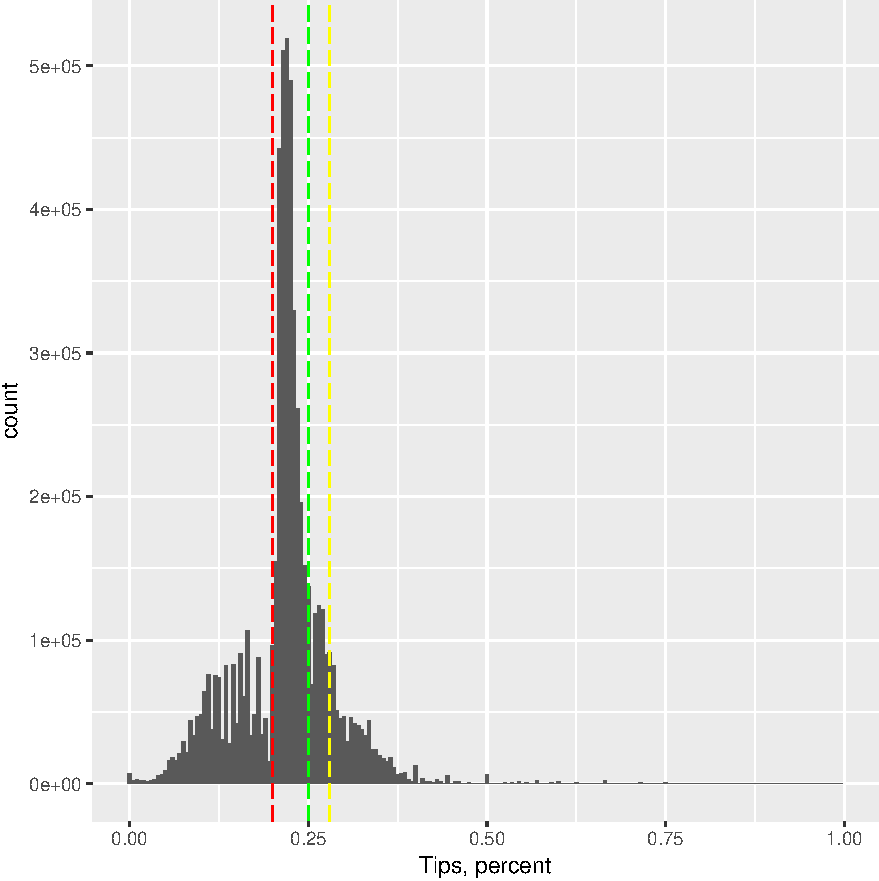
\includegraphics{thesis_files/figure-latex/tip-individual-1.pdf}
\caption{\label{fig:tip-individual}this is my caption}
\end{figure}
\subsection{Aggregated Zone-level Tip
Information}\label{aggregated-zone-level-tip-information}

Instead of studying factors that affect individual trips' percent tip,
it is more useful to study the aggregated effect of each zone on percent
tip.
\begin{Shaded}
\begin{Highlighting}[]
\KeywordTok{data}\NormalTok{(taxi_zone_lookup)}
\end{Highlighting}
\end{Shaded}
Taxi drivers are required to be indifferent to where passengers are
going. Therefore, it makes sense to investigate the average amount of
tips paid for each pick-up zone. What are the taxi pick-up zones that
have the highest tip percents?

We first calculate the average percent tip paid for each pick-up zone.
Here is a list of pick-up zones with more than 1000 trip per month along
with their average percent tip:
\begin{Shaded}
\begin{Highlighting}[]
\NormalTok{tip_pickup <-}\StringTok{ }\NormalTok{yellow_}\FloatTok{2016.}\NormalTok{08_tip }\OperatorTok\StringTok{ }\KeywordTok{group_by}\NormalTok{(PULocationID) }\OperatorTok\StringTok{ }
\StringTok{    }\KeywordTok{summarise}\NormalTok{(}\DataTypeTok{avg_tip =} \KeywordTok{mean}\NormalTok{(tip_perct), }\DataTypeTok{num_trips =} \KeywordTok{n}\NormalTok{(), }
        \DataTypeTok{avg_dis =} \KeywordTok{mean}\NormalTok{(trip_distance)) }\OperatorTok\StringTok{ }\KeywordTok{rename}\NormalTok{(}\DataTypeTok{LocationID =}\NormalTok{ PULocationID) }\OperatorTok\StringTok{ }
\StringTok{    }\KeywordTok{left_join}\NormalTok{(taxi_zone_lookup, }\DataTypeTok{by =} \StringTok{"LocationID"}\NormalTok{) }\OperatorTok\StringTok{ }
\StringTok{    }\KeywordTok{arrange}\NormalTok{(}\KeywordTok{desc}\NormalTok{(avg_tip)) }\OperatorTok\StringTok{ }\KeywordTok{filter}\NormalTok{(Zone }\OperatorTok{!=}\StringTok{ "Unknown"}\NormalTok{)}
\NormalTok{tip_pickup }\OperatorTok\StringTok{ }\KeywordTok{filter}\NormalTok{(num_trips }\OperatorTok{>}\StringTok{ }\DecValTok{1000}\NormalTok{) }\OperatorTok\StringTok{ }\KeywordTok{head}\NormalTok{(}\DecValTok{10}\NormalTok{)}
\end{Highlighting}
\end{Shaded}
\begin{verbatim}
# A tibble: 10 x 6
   LocationID   avg_tip num_trips  avg_dis   Borough
        <int>     <dbl>     <int>    <dbl>    <fctr>
 1        106 0.2343283      1088 3.600248  Brooklyn
 2        223 0.2335789      3014 4.212296    Queens
 3         37 0.2318139      2309 3.251091  Brooklyn
 4         80 0.2290748      4547 3.212947  Brooklyn
 5        189 0.2286701      1842 3.361069  Brooklyn
 6        112 0.2278641      3709 3.335044  Brooklyn
 7          7 0.2277946      7277 3.397217    Queens
 8         40 0.2275125      3537 4.186876  Brooklyn
 9         36 0.2271561      1334 3.571627  Brooklyn
10        230 0.2267445    171017 3.044212 Manhattan
# ... with 1 more variables: Zone <fctr>
\end{verbatim}
Below is a histogram of average percent tips paid for all pick-up zones.
As show on the plot, the first peak is around 20\%, which is the
cheapest default option on the touch panel for passengers to chose.
\begin{Shaded}
\begin{Highlighting}[]
\NormalTok{pickup_vis <-}\StringTok{ }\KeywordTok{ggplot}\NormalTok{(}\DataTypeTok{data =}\NormalTok{ tip_pickup, }\KeywordTok{aes}\NormalTok{(}\DataTypeTok{x =}\NormalTok{ avg_tip)) }\OperatorTok{+}\StringTok{ }
\StringTok{    }\KeywordTok{xlab}\NormalTok{(}\StringTok{"Tips, percent"}\NormalTok{) }\OperatorTok{+}\StringTok{ }\KeywordTok{geom_histogram}\NormalTok{(}\DataTypeTok{binwidth =} \FloatTok{0.005}\NormalTok{) }\OperatorTok{+}\StringTok{ }
\StringTok{    }\KeywordTok{geom_vline}\NormalTok{(}\DataTypeTok{xintercept =} \KeywordTok{c}\NormalTok{(}\FloatTok{0.2}\NormalTok{), }\DataTypeTok{col =} \StringTok{"red"}\NormalTok{, }\DataTypeTok{linetype =} \StringTok{"longdash"}\NormalTok{) }\OperatorTok{+}\StringTok{ }
\StringTok{    }\KeywordTok{geom_vline}\NormalTok{(}\DataTypeTok{xintercept =} \KeywordTok{c}\NormalTok{(}\FloatTok{0.25}\NormalTok{), }\DataTypeTok{col =} \StringTok{"green"}\NormalTok{, }
        \DataTypeTok{linetype =} \StringTok{"longdash"}\NormalTok{) }\OperatorTok{+}\StringTok{ }\KeywordTok{geom_vline}\NormalTok{(}\DataTypeTok{xintercept =} \KeywordTok{c}\NormalTok{(}\FloatTok{0.28}\NormalTok{), }
    \DataTypeTok{col =} \StringTok{"yellow"}\NormalTok{, }\DataTypeTok{linetype =} \StringTok{"longdash"}\NormalTok{) }\OperatorTok{+}\StringTok{ }\KeywordTok{scale_x_continuous}\NormalTok{(}\DataTypeTok{limits =} \KeywordTok{c}\NormalTok{(}\DecValTok{0}\NormalTok{, }
    \FloatTok{0.5}\NormalTok{))}
\NormalTok{pickup_vis}
\end{Highlighting}
\end{Shaded}
\begin{verbatim}
Warning: Removed 3 rows containing non-finite values (stat_bin).
\end{verbatim}
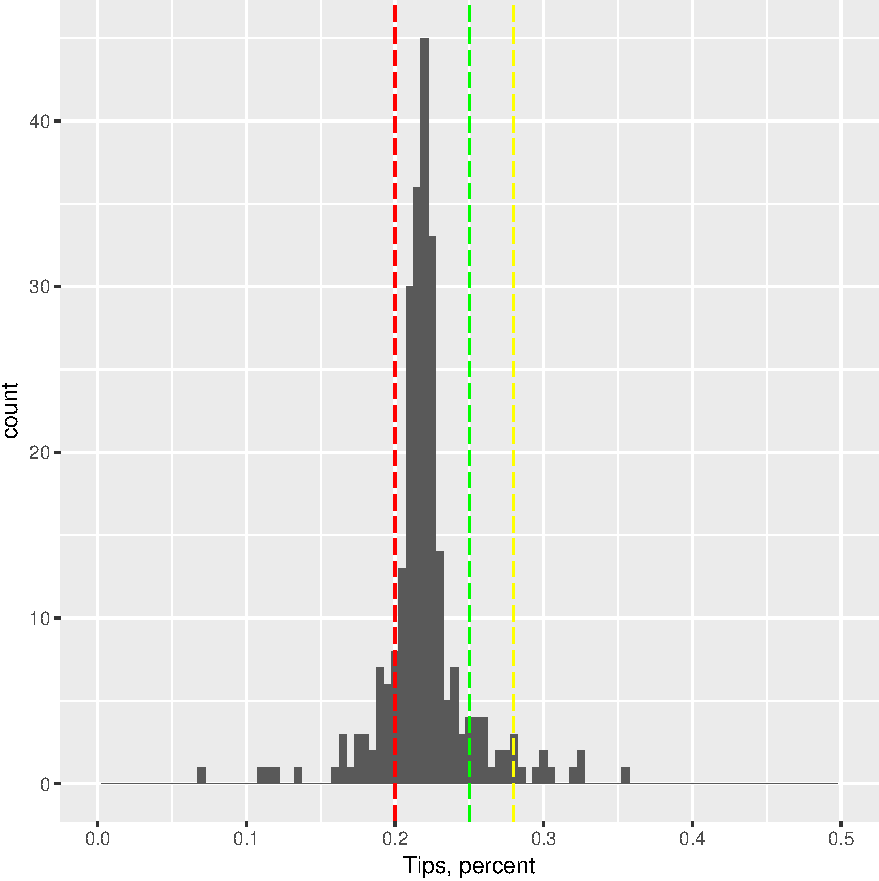
\includegraphics{thesis_files/figure-latex/unnamed-chunk-9-1.pdf}
\begin{Shaded}
\begin{Highlighting}[]
\NormalTok{tip_region <-}\StringTok{ }\NormalTok{yellow_}\FloatTok{2016.}\NormalTok{08_tip }\OperatorTok\StringTok{ }\KeywordTok{group_by}\NormalTok{(PULocationID, }
\NormalTok{    DOLocationID) }\OperatorTok\StringTok{ }\KeywordTok{summarise}\NormalTok{(}\DataTypeTok{avg_tip =} \KeywordTok{mean}\NormalTok{(tip_perct), }
    \DataTypeTok{trips =} \KeywordTok{n}\NormalTok{(), }\DataTypeTok{avg_dis =} \KeywordTok{mean}\NormalTok{(trip_distance)) }\OperatorTok\StringTok{ }
\StringTok{    }\CommentTok{# filter(trips > 10) %>%}
\KeywordTok{arrange}\NormalTok{(}\KeywordTok{desc}\NormalTok{(avg_tip)) }\OperatorTok\StringTok{ }\KeywordTok{rename}\NormalTok{(}\DataTypeTok{LocationID =}\NormalTok{ PULocationID) }\OperatorTok\StringTok{ }
\StringTok{    }\KeywordTok{left_join}\NormalTok{(taxi_zone_lookup, }\DataTypeTok{by =} \StringTok{"LocationID"}\NormalTok{)}
\CommentTok{# zone}
\NormalTok{region_vis <-}\StringTok{ }\NormalTok{pickup_vis }\OperatorTok\StringTok{ }\NormalTok{tip_region}
\NormalTok{region_vis}
\end{Highlighting}
\end{Shaded}
\begin{verbatim}
Warning: Removed 95 rows containing non-finite values (stat_bin).
\end{verbatim}
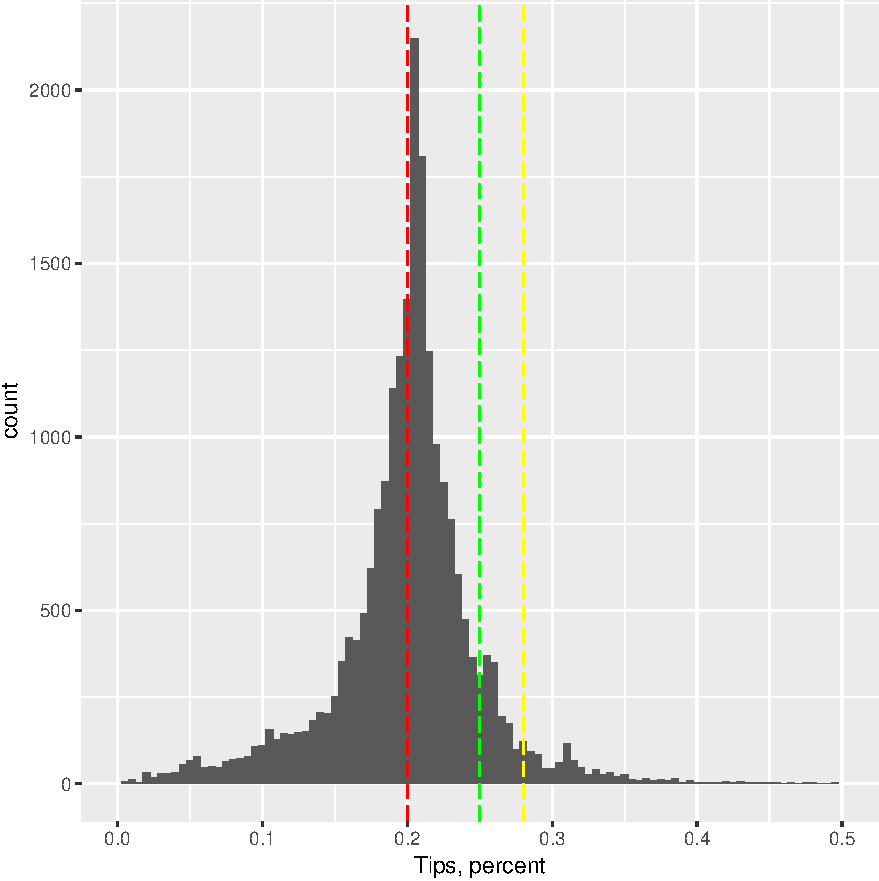
\includegraphics{thesis_files/figure-latex/unnamed-chunk-10-1.pdf} The
20\% peak is more clearly shown when we calculate the percent tips for
each pick-up and drop-off locatins pair instead of pick-up location
only.

\textbf{Does trip distance increase the percent tips paid?} One of the
questions that I always wonder is whether longer trips result in higher
tip percent. It takes taxi drivers more time to complete longer trips,
so passengers might want to compensate taxi drivers more. I personally
pay higher percent of tips for longer rides, so I believe trip distance
has an impact on percentage of tips paid.
\begin{Shaded}
\begin{Highlighting}[]
\NormalTok{tip_distance <-}\StringTok{ }\KeywordTok{lm}\NormalTok{(avg_tip }\OperatorTok{~}\StringTok{ }\NormalTok{avg_dis }\OperatorTok{+}\StringTok{ }\NormalTok{LocationID }\OperatorTok{+}\StringTok{ }
\StringTok{    }\NormalTok{DOLocationID, }\DataTypeTok{data =}\NormalTok{ tip_region)}
\KeywordTok{summary}\NormalTok{(tip_distance)}\OperatorTok{$}\NormalTok{coef[}\DecValTok{1}\OperatorTok{:}\DecValTok{2}\NormalTok{, ]}
\end{Highlighting}
\end{Shaded}
\begin{verbatim}
                 Estimate   Std. Error     t value  Pr(>|t|)
(Intercept)  2.025175e-01 1.140007e-03 177.6457606 0.0000000
avg_dis     -3.083442e-07 1.565416e-06  -0.1969727 0.8438507
\end{verbatim}
Acoording to the simple linear regression result, trip distance does not
have significant impact on the percent of tips paid, controlling for
both pick-up and drop-off locations.

\subsection{Which zones have the highest percent
tip?}\label{which-zones-have-the-highest-percent-tip}

Let's fist take a look at which pick-up zones have the highest number of
pickups. We create a heat map to visulizae the number of trip for each
pick-up zones on a map of New York City Taxi Zones.
\begin{Shaded}
\begin{Highlighting}[]
\KeywordTok{data}\NormalTok{(}\StringTok{"taxi_zones"}\NormalTok{)}
\KeywordTok{library}\NormalTok{(sp)}
\end{Highlighting}
\end{Shaded}
\begin{verbatim}
Warning: package 'sp' was built under R version 3.4.3
\end{verbatim}
\begin{Shaded}
\begin{Highlighting}[]
\NormalTok{pick_up_zones <-}\StringTok{ }\KeywordTok{merge}\NormalTok{(taxi_zones, tip_pickup, }\DataTypeTok{by.x =} \StringTok{"LocationID"}\NormalTok{, }
    \DataTypeTok{by.y =} \StringTok{"LocationID"}\NormalTok{)}
\end{Highlighting}
\end{Shaded}
\begin{Shaded}
\begin{Highlighting}[]
\KeywordTok{library}\NormalTok{(leaflet)}
\NormalTok{reds =}\StringTok{ }\KeywordTok{colorNumeric}\NormalTok{(}\StringTok{"Reds"}\NormalTok{, }\DataTypeTok{domain =} \OtherTok{NULL}\NormalTok{)}
\CommentTok{# leaflet(data = pick_up_zones) %>% addTiles() %>%}
\CommentTok{# addPolygons(fillColor = ~reds(num_trips),}
\CommentTok{# fillOpacity = 0.6, weight = 1, opacity = 0.8) %>%}
\CommentTok{# setView(lat = 40.7128, lng = -74.0060, zoom = 10)}
\end{Highlighting}
\end{Shaded}
It's obbivous that Manhattan, La Guardia Airport, and JKF Airport have
the most number of pick-ups.

Most yellow cab pick-ups occur in Manhattan. If we focus on the pick-up
zones that have more than 900 trips per month or 30 trips per day, then
we observe that many pick-up zones that have the highest percent tips
are in Brooklyn.
\begin{Shaded}
\begin{Highlighting}[]
\CommentTok{# pick a threshold for the cutoff number of trips}
\NormalTok{pickup_zone_}\DecValTok{900}\NormalTok{ <-}\StringTok{ }\NormalTok{tip_pickup }\OperatorTok\StringTok{ }\KeywordTok{filter}\NormalTok{(num_trips }\OperatorTok{>=}\StringTok{ }
\StringTok{    }\DecValTok{900}\NormalTok{) }\OperatorTok\StringTok{ }\KeywordTok{arrange}\NormalTok{(}\KeywordTok{desc}\NormalTok{(avg_tip))}

\NormalTok{pickup_zone_}\DecValTok{900} \OperatorTok\StringTok{ }\KeywordTok{head}\NormalTok{(}\DecValTok{10}\NormalTok{)}
\end{Highlighting}
\end{Shaded}
\begin{verbatim}
# A tibble: 10 x 6
   LocationID   avg_tip num_trips  avg_dis   Borough
        <int>     <dbl>     <int>    <dbl>    <fctr>
 1        106 0.2343283      1088 3.600248  Brooklyn
 2        223 0.2335789      3014 4.212296    Queens
 3         37 0.2318139      2309 3.251091  Brooklyn
 4         80 0.2290748      4547 3.212947  Brooklyn
 5        189 0.2286701      1842 3.361069  Brooklyn
 6        112 0.2278641      3709 3.335044  Brooklyn
 7          7 0.2277946      7277 3.397217    Queens
 8         40 0.2275125      3537 4.186876  Brooklyn
 9         36 0.2271561      1334 3.571627  Brooklyn
10        230 0.2267445    171017 3.044212 Manhattan
# ... with 1 more variables: Zone <fctr>
\end{verbatim}
\begin{Shaded}
\begin{Highlighting}[]
\CommentTok{# library(knitr) kable(pickup_zone_1000[1:10,2:6],}
\CommentTok{# caption = 'Taxi zone with the highest tip}
\CommentTok{# percent, threshold = 1000')}
\end{Highlighting}
\end{Shaded}
People might think it is more reasonable to ses a list that is populated
with Zones in Manhattan, since that's where all the wealthy people live.
However, it turns out that passengers who get on taxis in Brooklyn pays
more tips.

If we focus on the pick-up zones that have more than 90000 trips per
month or 3000 trips per day, then we observe that all pick-up zones that
have the highest percent tips are in Manhattan besides La Guardia
Airport.
\begin{Shaded}
\begin{Highlighting}[]
\CommentTok{# pick a threshold for the cutoff of number of}
\CommentTok{# trips}
\NormalTok{pickup_zone_}\DecValTok{90000}\NormalTok{ <-}\StringTok{ }\NormalTok{tip_pickup }\OperatorTok\StringTok{ }\KeywordTok{filter}\NormalTok{(num_trips }\OperatorTok{>=}\StringTok{ }
\StringTok{    }\DecValTok{90000}\NormalTok{) }\OperatorTok\StringTok{ }\KeywordTok{arrange}\NormalTok{(}\KeywordTok{desc}\NormalTok{(avg_tip))}
\NormalTok{pickup_zone_}\DecValTok{90000} \OperatorTok\StringTok{ }\KeywordTok{head}\NormalTok{(}\DecValTok{10}\NormalTok{)}
\end{Highlighting}
\end{Shaded}
\begin{verbatim}
# A tibble: 10 x 6
   LocationID   avg_tip num_trips   avg_dis   Borough
        <int>     <dbl>     <int>     <dbl>    <fctr>
 1        230 0.2267445    171017  3.044212 Manhattan
 2        186 0.2249650    213759  2.399181 Manhattan
 3        138 0.2249391    177262 10.084311    Queens
 4        161 0.2245180    230968  2.533839 Manhattan
 5        100 0.2245116    115242  2.467806 Manhattan
 6        162 0.2237261    224543  2.578228 Manhattan
 7        237 0.2226464    193035  1.942023 Manhattan
 8         48 0.2226313    180209  2.576908 Manhattan
 9        239 0.2224459    134925  2.454595 Manhattan
10        163 0.2218928    152459  2.556783 Manhattan
# ... with 1 more variables: Zone <fctr>
\end{verbatim}
\begin{Shaded}
\begin{Highlighting}[]
\CommentTok{# kable(pickup_zone_10000[1:10,2:5], caption =}
\CommentTok{# 'Taxi zone with the highest tip percent,}
\CommentTok{# threshold = 10000')}
\end{Highlighting}
\end{Shaded}
There are more than 100 times more yellow cab pick-ups that happen in
Manhattan everyday than in Brooklyn, and that is why there are many
dense red-shade polygons in the visulization above.

\subsection{Do taxi drivers tend to go to zones that offer high
tips?}\label{do-taxi-drivers-tend-to-go-to-zones-that-offer-high-tips}

So far, we have learned what pick-up zones offer the highest percent
tip. Now, we want to dig into the relationships between percent tip and
taxi-zone-specific variables.

It is not easy to find an available taxi on the street on New York City,
because the demand for taxi trips is much higher than the supply. Does
paying more tips help customers to more easily get taxis? If customers
from certain regions keep paying higher tips, taxi drivers might be able
to learn from their experiences in those regions, and be more willing to
wonder around those regions more often and pick up passengers. Pick-up
zones with higher tips should attract more taxi drivers with the control
of taxi zones. Let's test it out and see whether it is true:
\begin{Shaded}
\begin{Highlighting}[]
\NormalTok{tip_region}\OperatorTok{$}\NormalTok{LocationID <-}\StringTok{ }\KeywordTok{as.character}\NormalTok{(tip_region}\OperatorTok{$}\NormalTok{LocationID)}
\NormalTok{tip_pickup}\OperatorTok{$}\NormalTok{LocationID <-}\StringTok{ }\KeywordTok{as.character}\NormalTok{(tip_pickup}\OperatorTok{$}\NormalTok{LocationID)}
\NormalTok{tip_and_trip_}\DecValTok{1}\NormalTok{ <-}\StringTok{ }\KeywordTok{lm}\NormalTok{(trips }\OperatorTok{~}\StringTok{ }\NormalTok{avg_tip }\OperatorTok{+}\StringTok{ }\NormalTok{LocationID, }
    \DataTypeTok{data =}\NormalTok{ tip_region)}
\CommentTok{# summary(tip_and_trip_1)}
\KeywordTok{summary}\NormalTok{(tip_and_trip_}\DecValTok{1}\NormalTok{)}\OperatorTok{$}\NormalTok{coef[}\DecValTok{1}\OperatorTok{:}\DecValTok{2}\NormalTok{, ]}
\end{Highlighting}
\end{Shaded}
\begin{verbatim}
             Estimate Std. Error    t value     Pr(>|t|)
(Intercept) -188.5729   598.5170 -0.3150669 7.527139e-01
avg_tip     1447.2714   116.1562 12.4596964 1.629761e-35
\end{verbatim}
Each one percent increase in average tips in pick-up zones is associated
with 1447.2714 increase in the number of trips per month, controlling
the pick-up zone.
\begin{Shaded}
\begin{Highlighting}[]
\DecValTok{9942263}\OperatorTok{/}\DecValTok{31}
\end{Highlighting}
\end{Shaded}
\begin{verbatim}
[1] 320718.2
\end{verbatim}
\begin{Shaded}
\begin{Highlighting}[]
\FloatTok{1447.2714}\OperatorTok{/}\DecValTok{31}
\end{Highlighting}
\end{Shaded}
\begin{verbatim}
[1] 46.68617
\end{verbatim}
In August 2016, yellow cabs made an average of 320,718 daily trips.
Additionally, each one percent increase in average tips in pick-up zones
is associated with 47 increase in the number of trips per day in a
specific pick-up zone.

\subsection{Which pick-up zone has the highest price per
minute?}\label{which-pick-up-zone-has-the-highest-price-per-minute}

New York City Taxi Fare \& Limousine Commission has information on how
New York City taxi fare amount is calculated on their
\href{http://www.nyc.gov/html/tlc/html/passenger/taxicab_rate.shtml}{official
website}.

\textbf{Metered Fare Information} \textbf{Onscreen rate is `Rate \#01 --
Standard City Rate.'} \emph{The initial charge is \$2.50. }Plus 50 cents
per 1/5 mile or 50 cents per 60 seconds in slow traffic or when the
vehicle is stopped. \emph{In moving traffic on Manhattan streets, the
meter should ``click'' approximately every four downtown blocks, or one
block going cross-town (East-West). }There is a 50-cent MTA State
Surcharge for all trips that end in New York City or Nassau, Suffolk,
Westchester, Rockland, Dutchess, Orange or Putnam Counties. \emph{There
is a 30-cent Improvement Surcharge. }There is a daily 50-cent surcharge
from 8pm to 6am. \emph{There is a \$1 surcharge from 4pm to 8pm on
weekdays, excluding holidays. }Passengers must pay all bridge and tunnel
tolls. \emph{Your receipt will show your total fare including tolls.
Please take your receipt. }The driver is not required to accept bills
over \$20. \emph{Please tip your driver for safety and good service.
}There are no charges for extra passengers or bags.

In taxi fare calculation, the only unknown variable is slow-trafice
time, and all other variables were collected by the meters installed on
each medallion taxi for each trip. It is reasonable to assume that for
trips with the same pick-up and drop-off locations, the longer the total
slow traffic time is, the longer the trip would take. Taxi drivers are
compensated for both the normal-speed trip distance and the time spent
in slow-traffice. According to the fare calculation algorithm, in moving
traffic on Manhattan streets, the meter should ``click'' approximately
every four downtown blocks, or one block going cross-town (East-West);
in slow traffic, the meter should ``click'' every 60 seconds. Therefore,
slow traffic reduces the fare per minute ratio.

New York CIty has the worst traffic jam, and it has overtaken Miami to
be voted the U.S. city with the angriest and most aggressive drivers in
2009, according to a survey on road rage released on Tuesday. Bad
traffic also cause slow-traffic, and taxi drivers tend to suck in
traffic during rush hours. Does fare per minute ratio have an impact on
the percent tip that passengers pay? Do passengers compensate taxi
drivers more during rush hours? Are passengers sympathetic to taxi
drivers for the time they spend in slow traffic?

\url{https://www.reuters.com/article/us-driving-roadrage-life/new-york-drivers-named-most-aggressive-angry-in-u-s-idUSTRE55F1J720090616}
\begin{Shaded}
\begin{Highlighting}[]
\KeywordTok{library}\NormalTok{(lubridate)}
\NormalTok{yellow_}\FloatTok{2016.}\NormalTok{08_time <-}\StringTok{ }\NormalTok{yellow_}\FloatTok{2016.}\NormalTok{08_tip }\OperatorTok\StringTok{ }\KeywordTok{mutate}\NormalTok{(}\DataTypeTok{duration =} \KeywordTok{round}\NormalTok{((tpep_dropoff_datetime }\OperatorTok{-}\StringTok{ }
\StringTok{    }\NormalTok{tpep_pickup_datetime)}\OperatorTok{/}\DecValTok{60}\NormalTok{, }\DecValTok{2}\NormalTok{)) }\OperatorTok\StringTok{ }\KeywordTok{mutate}\NormalTok{(}\DataTypeTok{duration =} \KeywordTok{as.numeric}\NormalTok{(duration)) }\OperatorTok\StringTok{ }
\StringTok{    }\KeywordTok{filter}\NormalTok{(duration }\OperatorTok{>}\StringTok{ }\DecValTok{0}\NormalTok{) }\OperatorTok\StringTok{ }\KeywordTok{mutate}\NormalTok{(}\DataTypeTok{fare_per_min =}\NormalTok{ fare_amount}\OperatorTok{/}\NormalTok{duration)}

\CommentTok{# summary(yellow_2016.08_time$fare_per_min)}
\NormalTok{fare_min_ratio <-}\StringTok{ }\KeywordTok{lm}\NormalTok{(tip_perct }\OperatorTok{~}\StringTok{ }\NormalTok{fare_per_min, }\DataTypeTok{data =}\NormalTok{ yellow_}\FloatTok{2016.}\NormalTok{08_time)}
\KeywordTok{summary}\NormalTok{(fare_min_ratio)}
\end{Highlighting}
\end{Shaded}
\begin{verbatim}

Call:
lm(formula = tip_perct ~ fare_per_min, data = yellow_2016.08_time)

Residuals:
     Min       1Q   Median       3Q      Max 
-0.21882 -0.01891  0.00242  0.02685  0.77849 

Coefficients:
               Estimate Std. Error t value Pr(>|t|)    
(Intercept)   2.189e-01  2.815e-05 7776.48   <2e-16 ***
fare_per_min -1.785e-05  6.984e-07  -25.56   <2e-16 ***
---
Signif. codes:  0 '***' 0.001 '**' 0.01 '*' 0.05 '.' 0.1 ' ' 1

Residual standard error: 0.06937 on 6088066 degrees of freedom
Multiple R-squared:  0.0001073, Adjusted R-squared:  0.0001071 
F-statistic: 653.2 on 1 and 6088066 DF,  p-value: < 2.2e-16
\end{verbatim}
As shown in the regression result, fare per minute ratio has a
significant negative impact on percent tip. Since having more slow
traffic time spent on the road reduces the fare per minute ratio, slow
traffice does increase the impact on percent tip. Passengers do pay more
tips to taxi drivers during rush hours.

\chapter{New York City Taxi Consumer}\label{chapter3}

\section{How long does it take for passengers to get to JFK, LaGuardia,
and Newark Airports? When is the best time to
travel?}\label{how-long-does-it-take-for-passengers-to-get-to-jfk-laguardia-and-newark-airports-when-is-the-best-time-to-travel}
\begin{Shaded}
\begin{Highlighting}[]
\KeywordTok{library}\NormalTok{(dplyr)}
\KeywordTok{library}\NormalTok{(readr)}
\NormalTok{yellow_}\FloatTok{2015.}\NormalTok{08_cleaned <-}\StringTok{ }\KeywordTok{read_csv}\NormalTok{(}\StringTok{"~/Desktop/Honors Thesis/thesis/index/data/yellow_tripdata_2015-08.csv"}\NormalTok{)}
\NormalTok{yellow_}\FloatTok{2016.}\NormalTok{08_tip <-}\StringTok{ }\NormalTok{yellow_}\FloatTok{2015.}\NormalTok{08_cleaned }\OperatorTok\StringTok{ }\KeywordTok{filter}\NormalTok{(fare_amount }\OperatorTok{>}\StringTok{ }
\StringTok{    }\DecValTok{0}\NormalTok{) }\OperatorTok\StringTok{ }\KeywordTok{filter}\NormalTok{(tip_amount }\OperatorTok{>}\StringTok{ }\DecValTok{0}\NormalTok{) }\OperatorTok\StringTok{ }\KeywordTok{filter}\NormalTok{(PULocationID }\OperatorTok{!=}\StringTok{ }
\StringTok{    }\NormalTok{DOLocationID)}
\end{Highlighting}
\end{Shaded}
\begin{Shaded}
\begin{Highlighting}[]
\NormalTok{dataset }\OperatorTok\StringTok{ }\KeywordTok{group_by}\NormalTok{()}
\end{Highlighting}
\end{Shaded}
\section{How does weather affect New York City taxi and Uber trips? How
does snowfall affect taxi and Uber
trips?}\label{how-does-weather-affect-new-york-city-taxi-and-uber-trips-how-does-snowfall-affect-taxi-and-uber-trips}

\chapter{New York City Taxi Fare \& Limousine
Commission}\label{chapter4}

\section{Should there be a flat rate between Manhattan and the JFK
Airport?}\label{should-there-be-a-flat-rate-between-manhattan-and-the-jfk-airport}

\subsection{People in Manhattan benefit from the \$52 flat
rate.}\label{people-in-manhattan-benefit-from-the-52-flat-rate.}

Why is there a flat rate to and from JFK airport and any location in
Manhattan? Why is the flat rate \$52? Does TLC make profit from the \$52
flat rate? Does \$52 reduce the cogestion on the road to JFK airport and
make taking a train a more preferable choice?

If there is no flat rate between JFK and Manhattan,
\begin{Shaded}
\begin{Highlighting}[]
\NormalTok{jfk_trip <-}\StringTok{ }\NormalTok{yellow_}\FloatTok{2016.}\NormalTok{08_cleaned }\OperatorTok\StringTok{ }\KeywordTok{filter}\NormalTok{(RatecodeID }\OperatorTok{==}\StringTok{ }
\StringTok{    }\DecValTok{2}\NormalTok{) }\OperatorTok\StringTok{ }\KeywordTok{filter}\NormalTok{(payment_type }\OperatorTok{!=}\StringTok{ }\DecValTok{3}\NormalTok{) }\OperatorTok\StringTok{ }\KeywordTok{filter}\NormalTok{(trip_distance }\OperatorTok{>}\StringTok{ }
\StringTok{    }\DecValTok{0}\NormalTok{) }\OperatorTok\StringTok{ }\KeywordTok{filter}\NormalTok{(fare_amount }\OperatorTok{>}\StringTok{ }\DecValTok{0}\NormalTok{) }\OperatorTok\StringTok{ }\KeywordTok{filter}\NormalTok{(PULocationID }\OperatorTok{!=}\StringTok{ }
\StringTok{    }\NormalTok{DOLocationID) }\OperatorTok\StringTok{ }\KeywordTok{mutate}\NormalTok{(}\DataTypeTok{est_fare =} \FloatTok{2.5} \OperatorTok{+}\StringTok{ }\FloatTok{0.5} \OperatorTok{*}\StringTok{ }
\StringTok{    }\NormalTok{trip_distance }\OperatorTok{*}\StringTok{ }\DecValTok{5} \OperatorTok{+}\StringTok{ }\NormalTok{extra }\OperatorTok{+}\StringTok{ }\NormalTok{improvement_surcharge }\OperatorTok{+}\StringTok{ }
\StringTok{    }\NormalTok{mta_tax }\OperatorTok{+}\StringTok{ }\NormalTok{tolls_amount, }\DataTypeTok{est_diff =}\NormalTok{ est_fare }\OperatorTok{-}\StringTok{ }\NormalTok{fare_amount)}

\NormalTok{to_jfk <-}\StringTok{ }\NormalTok{jfk_trip }\OperatorTok\StringTok{ }\KeywordTok{filter}\NormalTok{(DOLocationID }\OperatorTok{==}\StringTok{ }\DecValTok{132}\NormalTok{)}
\end{Highlighting}
\end{Shaded}
\begin{Shaded}
\begin{Highlighting}[]
\NormalTok{to_jkf_zone <-}\StringTok{ }\NormalTok{to_jfk }\OperatorTok\StringTok{ }\KeywordTok{group_by}\NormalTok{(PULocationID) }\OperatorTok\StringTok{ }
\StringTok{    }\KeywordTok{summarise}\NormalTok{(}\DataTypeTok{num_trips =} \KeywordTok{n}\NormalTok{(), }\DataTypeTok{avg_dis =} \KeywordTok{mean}\NormalTok{(trip_distance), }
        \DataTypeTok{avg_fare =} \KeywordTok{mean}\NormalTok{(est_fare)) }\OperatorTok\StringTok{ }\KeywordTok{rename}\NormalTok{(}\DataTypeTok{LocationID =}\NormalTok{ PULocationID) }\OperatorTok\StringTok{ }
\StringTok{    }\KeywordTok{left_join}\NormalTok{(taxi_zone_lookup, }\DataTypeTok{by =} \StringTok{"LocationID"}\NormalTok{)}

\CommentTok{# to_jkf_fare <- merge(taxi_zones, to_jkf_zone,}
\CommentTok{# by.x = 'LocationID', by.y = 'PULocationID')}
\end{Highlighting}
\end{Shaded}
\begin{Shaded}
\begin{Highlighting}[]
\NormalTok{to_jkf_zone_above <-}\StringTok{ }\NormalTok{to_jkf_zone }\OperatorTok\StringTok{ }\KeywordTok{filter}\NormalTok{(Borough }\OperatorTok{==}\StringTok{ }
\StringTok{    "Manhattan"}\NormalTok{) }\OperatorTok\StringTok{ }\CommentTok{# filter(avg_fare >= 52) %>%}
\KeywordTok{arrange}\NormalTok{(}\KeywordTok{desc}\NormalTok{(avg_fare))}

\KeywordTok{kable}\NormalTok{(to_jkf_zone_above[}\DecValTok{1}\OperatorTok{:}\DecValTok{44}\NormalTok{, ], }\DataTypeTok{caption =} \StringTok{"Pick-up Zones with avergae fare to JKF Airport"}\NormalTok{)}
\end{Highlighting}
\end{Shaded}
\begin{table}

\caption{\label{tab:unnamed-chunk-23}Pick-up Zones with avergae fare to JKF Airport}
\centering
\begin{tabular}[t]{r|r|r|r|l|l}
\hline
LocationID & num\_trips & avg\_dis & avg\_fare & Borough & Zone\\
\hline
127 & 6 & 22.85833 & 65.06250 & Manhattan & Inwood\\
\hline
243 & 8 & 21.54250 & 63.82125 & Manhattan & Washington Heights North\\
\hline
13 & 1266 & 22.09787 & 62.44055 & Manhattan & Battery Park City\\
\hline
244 & 74 & 20.42216 & 60.27892 & Manhattan & Washington Heights South\\
\hline
239 & 1685 & 20.47249 & 60.11053 & Manhattan & Upper West Side South\\
\hline
261 & 723 & 21.22151 & 59.59012 & Manhattan & World Trade Center\\
\hline
143 & 655 & 20.53586 & 59.26524 & Manhattan & Lincoln Square West\\
\hline
238 & 1233 & 19.93394 & 59.02019 & Manhattan & Upper West Side North\\
\hline
12 & 41 & 20.62537 & 58.44146 & Manhattan & Battery Park\\
\hline
88 & 362 & 20.30909 & 57.79963 & Manhattan & Financial District South\\
\hline
151 & 637 & 19.39038 & 57.71180 & Manhattan & Manhattan Valley\\
\hline
116 & 67 & 19.27463 & 57.54149 & Manhattan & Hamilton Heights\\
\hline
158 & 751 & 19.68667 & 57.52564 & Manhattan & Meatpacking/West Village West\\
\hline
24 & 248 & 19.21508 & 57.20560 & Manhattan & Bloomingdale\\
\hline
152 & 67 & 19.12522 & 57.10769 & Manhattan & Manhattanville\\
\hline
236 & 1574 & 18.94848 & 56.57681 & Manhattan & Upper East Side North\\
\hline
166 & 447 & 18.88353 & 56.54928 & Manhattan & Morningside Heights\\
\hline
140 & 1005 & 18.90681 & 56.04591 & Manhattan & Lenox Hill East\\
\hline
262 & 1127 & 18.62596 & 55.91055 & Manhattan & Yorkville East\\
\hline
50 & 628 & 18.90573 & 55.50548 & Manhattan & Clinton West\\
\hline
263 & 1185 & 18.56361 & 55.47873 & Manhattan & Yorkville West\\
\hline
87 & 1252 & 19.67124 & 55.39298 & Manhattan & Financial District North\\
\hline
142 & 1832 & 19.19067 & 55.37192 & Manhattan & Lincoln Square East\\
\hline
246 & 591 & 18.24122 & 54.95910 & Manhattan & West Chelsea/Hudson Yards\\
\hline
42 & 92 & 18.05380 & 54.87038 & Manhattan & Central Harlem North\\
\hline
43 & 826 & 18.74347 & 54.85187 & Manhattan & Central Park\\
\hline
75 & 470 & 18.16949 & 54.77060 & Manhattan & East Harlem South\\
\hline
41 & 238 & 18.02353 & 54.33887 & Manhattan & Central Harlem\\
\hline
68 & 1623 & 17.91729 & 53.98436 & Manhattan & East Chelsea\\
\hline
231 & 947 & 19.36168 & 53.91387 & Manhattan & TriBeCa/Civic Center\\
\hline
249 & 866 & 18.50783 & 53.65980 & Manhattan & West Village\\
\hline
237 & 1493 & 18.42390 & 53.65730 & Manhattan & Upper East Side South\\
\hline
48 & 2780 & 17.99023 & 53.33922 & Manhattan & Clinton East\\
\hline
141 & 1197 & 18.23483 & 53.16414 & Manhattan & Lenox Hill West\\
\hline
90 & 1151 & 17.58740 & 53.09904 & Manhattan & Flatiron\\
\hline
230 & 6585 & 17.78133 & 52.99621 & Manhattan & Times Sq/Theatre District\\
\hline
74 & 257 & 17.28008 & 52.70712 & Manhattan & East Harlem North\\
\hline
186 & 2236 & 17.30646 & 52.66024 & Manhattan & Penn Station/Madison Sq West\\
\hline
113 & 947 & 17.94572 & 52.65996 & Manhattan & Greenwich Village North\\
\hline
125 & 430 & 18.69965 & 52.63090 & Manhattan & Hudson Sq\\
\hline
100 & 1742 & 17.24245 & 52.43794 & Manhattan & Garment District\\
\hline
234 & 1803 & 17.20495 & 52.42949 & Manhattan & Union Sq\\
\hline
105 & 1 & 17.31000 & 52.11500 & Manhattan & Governor's Island/Ellis Island/Liberty Island\\
\hline
224 & 315 & 17.46460 & 52.07268 & Manhattan & Stuy Town/Peter Cooper Village\\
\hline
\end{tabular}
\end{table}
Imagine it's your first time travelling to New York City, and you
decided to live in a hotel in Manhattan Since you do not know much about
the city, the \$52 flat rate is nice for you, and it incentivizes you to
take taxi to the JFK Airport. If there is no flat rate, there is
uncertainty in how much someone needs to pay to take a taxi to JFK, and
tourists might instead choose to take the train, even though taking a
train would cost them more time and inconvenience.

Additionally, people who are native to Manhattan would have paid more
than \$52 to take a taxi to go to the JFK Airport. The higher the taxi
fare is, the less the demand for taxi will be. Therefore, having a flat
rate,helps taxi drivers to get more trips from Manhattan to JFK Airport.

\section{However, are taxi drivers happy with the flat
rate?}\label{however-are-taxi-drivers-happy-with-the-flat-rate}

What the expected fare from JKF Airport to Manhattan?
\begin{Shaded}
\begin{Highlighting}[]
\NormalTok{from_jfk <-}\StringTok{ }\NormalTok{jfk_trip }\OperatorTok\StringTok{ }\KeywordTok{filter}\NormalTok{(PULocationID }\OperatorTok{==}\StringTok{ }\DecValTok{132}\NormalTok{)}

\NormalTok{from_jkf_zone <-}\StringTok{ }\NormalTok{from_jfk }\OperatorTok\StringTok{ }\KeywordTok{group_by}\NormalTok{(DOLocationID) }\OperatorTok\StringTok{ }
\StringTok{    }\KeywordTok{summarise}\NormalTok{(}\DataTypeTok{num_trips =} \KeywordTok{n}\NormalTok{(), }\DataTypeTok{avg_dis =} \KeywordTok{mean}\NormalTok{(trip_distance), }
        \DataTypeTok{avg_fare =} \KeywordTok{mean}\NormalTok{(est_fare)) }\OperatorTok\StringTok{ }\KeywordTok{rename}\NormalTok{(}\DataTypeTok{LocationID =}\NormalTok{ DOLocationID) }\OperatorTok\StringTok{ }
\StringTok{    }\KeywordTok{left_join}\NormalTok{(taxi_zone_lookup, }\DataTypeTok{by =} \StringTok{"LocationID"}\NormalTok{)}

\NormalTok{from_jkf_fare <-}\StringTok{ }\KeywordTok{merge}\NormalTok{(taxi_zones, from_jkf_zone, }\DataTypeTok{by.x =} \StringTok{"LocationID"}\NormalTok{, }
    \DataTypeTok{by.y =} \StringTok{"LocationID"}\NormalTok{)}

\CommentTok{# cols <- brewer.pal(n = 4, name = 'Greys')}
\NormalTok{lcols <-}\StringTok{ }\KeywordTok{cut}\NormalTok{(from_jkf_fare}\OperatorTok{$}\NormalTok{avg_fare, }\DataTypeTok{breaks =} \KeywordTok{quantile}\NormalTok{(from_jkf_fare}\OperatorTok{$}\NormalTok{avg_fare, }
    \DataTypeTok{na.rm =} \OtherTok{TRUE}\NormalTok{), }\DataTypeTok{labels =}\NormalTok{ cols)}
\KeywordTok{plot}\NormalTok{(from_jkf_fare, }\DataTypeTok{col =} \KeywordTok{as.character}\NormalTok{(lcols))}

\NormalTok{from_jkf_zone_above <-}\StringTok{ }\NormalTok{from_jkf_zone }\OperatorTok\StringTok{ }\KeywordTok{filter}\NormalTok{(Borough }\OperatorTok{==}\StringTok{ }
\StringTok{    "Manhattan"}\NormalTok{) }\OperatorTok\StringTok{ }\CommentTok{# filter(avg_fare >= 52) %>%}
\KeywordTok{arrange}\NormalTok{(}\KeywordTok{desc}\NormalTok{(avg_fare))}
\KeywordTok{kable}\NormalTok{(to_jkf_zone_above[}\DecValTok{1}\OperatorTok{:}\DecValTok{67}\NormalTok{, ], }\DataTypeTok{caption =} \StringTok{"Drop-off Zones with average fare amount from JFK Airport"}\NormalTok{)}
\end{Highlighting}
\end{Shaded}
how much time it would take for a cb driver to do a round trip
\url{https://ny.curbed.com/2017/1/17/14296892/yellow-taxi-nyc-uber-lyft-via-numbers}

\chapter{Conclusion}\label{chapter5}

\section{Future Research}\label{future-research}

For future study, I would love to investigate the sharp decline in the
consumption of NYC yellow cab after e-hail services were introduced into
the NYC ride-hail market. I also want to study what the impact of
introducing new GPS and entertainment system is on the number of rides.
The global product and marketing at Verifone, Jason Gross, said that,
``I like to say that we provide what Uber says it provides.'' With the
raised expectation among rides caused by Uber and Lyft, yellow taxi
industry need to respond quickly. How does the market react to the newly
installed entertainment system? Has the market share of yellow cab
rebounded since 2016? By looking into the patterns in market shares, it
might be possible for me to predict the future market share distribution
and find out what features of ride-hail transportation are the ones that
affect market share distribution the most.

\appendix

\chapter{The First Appendix}\label{the-first-appendix}

This first appendix includes all of the R chunks of code that were
hidden throughout the document (using the \texttt{include\ =\ FALSE}
chunk tag) to help with readibility and/or setup.

\textbf{In the main Rmd file}
\begin{Shaded}
\begin{Highlighting}[]
\CommentTok{# This chunk ensures that the thesisdown package is}
\CommentTok{# installed and loaded. This thesisdown package}
\CommentTok{# includes the template files for the thesis.}
\ControlFlowTok{if}\NormalTok{ (}\OperatorTok{!}\KeywordTok{require}\NormalTok{(devtools)) }\KeywordTok{install.packages}\NormalTok{(}\StringTok{"devtools"}\NormalTok{, }
    \DataTypeTok{repos =} \StringTok{"http://cran.rstudio.com"}\NormalTok{)}
\ControlFlowTok{if}\NormalTok{ (}\OperatorTok{!}\KeywordTok{require}\NormalTok{(thesisdown)) devtools}\OperatorTok{::}\KeywordTok{install_github}\NormalTok{(}\StringTok{"ismayc/thesisdown"}\NormalTok{)}
\KeywordTok{library}\NormalTok{(thesisdown)}
\end{Highlighting}
\end{Shaded}
\textbf{In Chapter \ref{ref-labels}:}

\chapter{The Second Appendix, for
Fun}\label{the-second-appendix-for-fun}

\backmatter

\chapter*{References}\label{references}
\addcontentsline{toc}{chapter}{References}

\markboth{References}{References}

\noindent

\setlength{\parindent}{-0.20in} \setlength{\leftskip}{0.20in}
\setlength{\parskip}{8pt}

\hypertarget{refs}{}
\hypertarget{ref-angel2000}{}
Angel, E. (2000). \emph{Interactive computer graphics : A top-down
approach with opengl}. Boston, MA: Addison Wesley Longman.

\hypertarget{ref-angel2001}{}
Angel, E. (2001a). \emph{Batch-file computer graphics : A bottom-up
approach with quicktime}. Boston, MA: Wesley Addison Longman.

\hypertarget{ref-angel2002a}{}
Angel, E. (2001b). \emph{Test second book by angel}. Boston, MA: Wesley
Addison Longman.


% Index?

\end{document}
